\chapter{High fidelity qutrit single-shot readout and reset} \label{ch:qutrit_readout}

As mentioned in Section \ref{sec:intro_building_qc}, information stored in qubits cannot be copied which prevents redundancy and majority voting as an error correcting scheme. Instead, fault-tolerant quantum computing requires quantum error correction codes~\cite{Gottesman2010AnComputation, DiVincenzo1996Fault-TolerantCodes} such as the surface code~\cite{Fowler2012SurfaceComputation}. 

However, standard decoders for the surface code typically assume there is no population leakage outside of the computational subspace spanned by the \0 and \1 states ~\cite{Ghosh2015}. Unfortunately, most physical implementation of qubits are multi-level systems (see Section \ref{sec:intro_building_qc}). Consequently, qubit manipulation occasionally results in \textit{leakage}, the phenomenon of populating levels beyond \0 or \1 which are not part of the computational basis. 

Detecting and calibrating low leakage gates requires accurate measurement of additional states of the qubit outside its computational basis. This appendix describes how we perform high-fidelity single-shot readout of the first 3 eigenstates of a transmon, respectively named $\ket{g}$ (ground state) or \0, $\ket{e}$ (first excited state) or \1, and $\ket{f}$ (second excited state) or \2. Higher levels are not considered the scope of this work but are further discussed in~\cite{Sank2016Measurement-InducedApproximation, ElderHigh-fidelityCircuits}.

The first section provides a theoretical description of the readout scheme and outlines the steps required to achieve high fidelity readout. In particular, we describe how to find the optimal readout frequency and derive the statistically optimal state discrimination procedure. The next section details the implementation of the scheme within our measurement framework.  Thereafter, we provide experimental data achieving a correct state assignment probability of 98.5\% and illustrate the scheme on a $T_1$ measurement of the \f{} level. Finally, the last section demonstrates that this high fidelity readout scheme can enable high quality three-level active reset of the transmon to the ground state.

\section{Three-level readout}
\label{s:high_level_description}
The state of a qutrit (the three-level extension of a qubit), $\ket{\psi}$, reads,
\begin{equation} \label{eq:qutrit_state}
    \ket{\psi} = \alpha_g \g + \alpha_1 \e + \alpha_f \f
\end{equation}
and is measured with probability $P_i = |\alpha_i|^2$ in $\ket{i}$ for $k \in \{g,e,f\}$. The probabilities $P_g$, $P_e$, $P_f$ are also referred as the ground state, first-excited and second-excited state populations respectively.

To readout the state of a qutrit, we make use of a dispersive interaction between the transmon and a resonator~\cite{Blais2004CavityComputation, Wallraff2005ApproachingReadout} which we probe with a voltage pulse. The output signal, $S_{\mathrm{out}}(t)$, consists of an in-phase real component, $I(t)$, and an imaginary quadrature, $Q(t)$,
\begin{equation}
    S_{\mathrm{out}}(t) = I(t) + \i Q(t)
\end{equation}
After several stages of amplification, we use the state-dependent time-response of the resonator $S_{\mathrm{out}}(t)$ to discriminate between the ground state, the first excited state and the second excited state.  

In average readout, the measurement is repeated many times and averaged to reduce noise. By contrast, the objective of single-shot readout is to construct a function acting on a single time trace $S_{\mathrm{out}}(t)$ to determine the projected state of the qutrit on one of its three eigenstates with high probability. 

With the approximation that the qutrit is perfectly prepared in one of its eigenstates, the projected state of the qutrit is assigned,
\begin{equation} \label{eq:max_likelihood_state}
    \ket{\psi_{proj}} = \ket{i'}
\end{equation}
where $i'$ is the most likely state label according to the state assignment model.
Repeated eigenstate preparation, measurement and state assignment yields statistics characterizing the readout performance conveniently visualized in the state assignment probability matrix,
\begin{equation}     \label{eq:state_assignment_probability_matrix}
A = \begin{pmatrix}
P(g \mid g) & P(e \mid g) & P(f \mid g) \\
P(g  \mid e) & P(e \mid e) & P(f \mid e)\\
P(g \mid f) &  P(e \mid f) &  P(f \mid f)\\
\end{pmatrix}
\end{equation}
where the element of row $i$ and column $j$ corresponds to $P(s_j|s_i)$, the estimate probability of assigning a prepared state $s_i$ to state $s_j$. These estimates are computed from the counts of the repeated single-shot measurements.

Under ideal conditions, $A$ coincides with the identity matrix. However, in practice several mechanisms prevent the assignment matrix of reaching identity. For instance, $T_1$ decay before and during the readout, readout errors due to finite \gls{snr}, thermal population and state preparation errors. 

We aim at achieving the highest average three-level readout and therefore choose to optimize the readout for the highest \gls{snr} between the 3 states concurrently. This corresponds to minimizing the readout overlap, $\epsilon$, defined as the averaged sum of the non-diagonal elements of the state assignment probability matrix\footnote{Note that specific experiments could benefit from other optimizations criteria. For instance, maximizing the minimum \gls{snr} between one state and the other two, which corresponds to maximizing the minimum value of the trace of $A$.},
\begin{equation} \label{eq:qutrit_readout_overlap}
    \epsilon = \frac{1}{3}\sum_{i=0}^{2}{\sum_{j \neq i}^{2}{P(s_j | s_i)}}
\end{equation}

$A$ is highly dependent on the readout pulse frequency. Therefore, we start by searching the readout frequency minimizing $\epsilon$.

\section{Readout frequency optimization} \label{s:frequency_optimization}
The time-response of the readout resonator depends not only on the qubit state but also the frequency of the readout pulse, $f$. Hence, we start by preparing the qutrit in \g, (respectively \e, \f) and measuring the time-integrated (with boxcar integration weights~\cite{Gambetta2007}) resonator response for a range of frequencies. The amplitude of each response is shown in Fig.~\ref{fig:qutrit_readout_ro_freq_opt}(a) as function of the readout pulse frequency.

The dominating noise sources in the readout are the amplifiers, which are independent of the measured state and subject to white noise over the considered frequency range. Hence, we model the noise for each state as frequency- and time-independent Gaussian white noise\footnote{T$_1$-decay introduces non-Gaussian noise which is not captured by this model. The effects of these phenomenon on the state assignment are discussed in Section \ref{s:experimental_data}.}. Due to the linearity of integration, the noise for each state in the integrated IQ-plane also follows a Gaussian distribution, centered at the average time-integrated resonator response for each frequency. We provide an example for $f = 6.890\unit{GHz}$ (indicated with a dashed, black line in Fig.~\ref{fig:qutrit_readout_ro_freq_opt}(a) and b) in Fig.~\ref{fig:qutrit_readout_ro_freq_opt}(c) where the three Gaussian distributions are centered at points $G$, $E$ and $F$ respectively.

The statistically optimal approach to assign a new data point to a state in this plane is a multi-modal \gls{gmm}~\cite{Bishop2006, Hastie2017, Reuer2018}.
With this model we compute the posterior probability of a new incoming data point to be produced by each eigenstate and assign it to the state with highest posterior probability~\cite{Lacroix2019} (i.e. maximum likelihood state assignment). The decision boundaries are the collection of points in space with equal likelihood for different distributions.

\begin{figure}[ht]
    \centering
    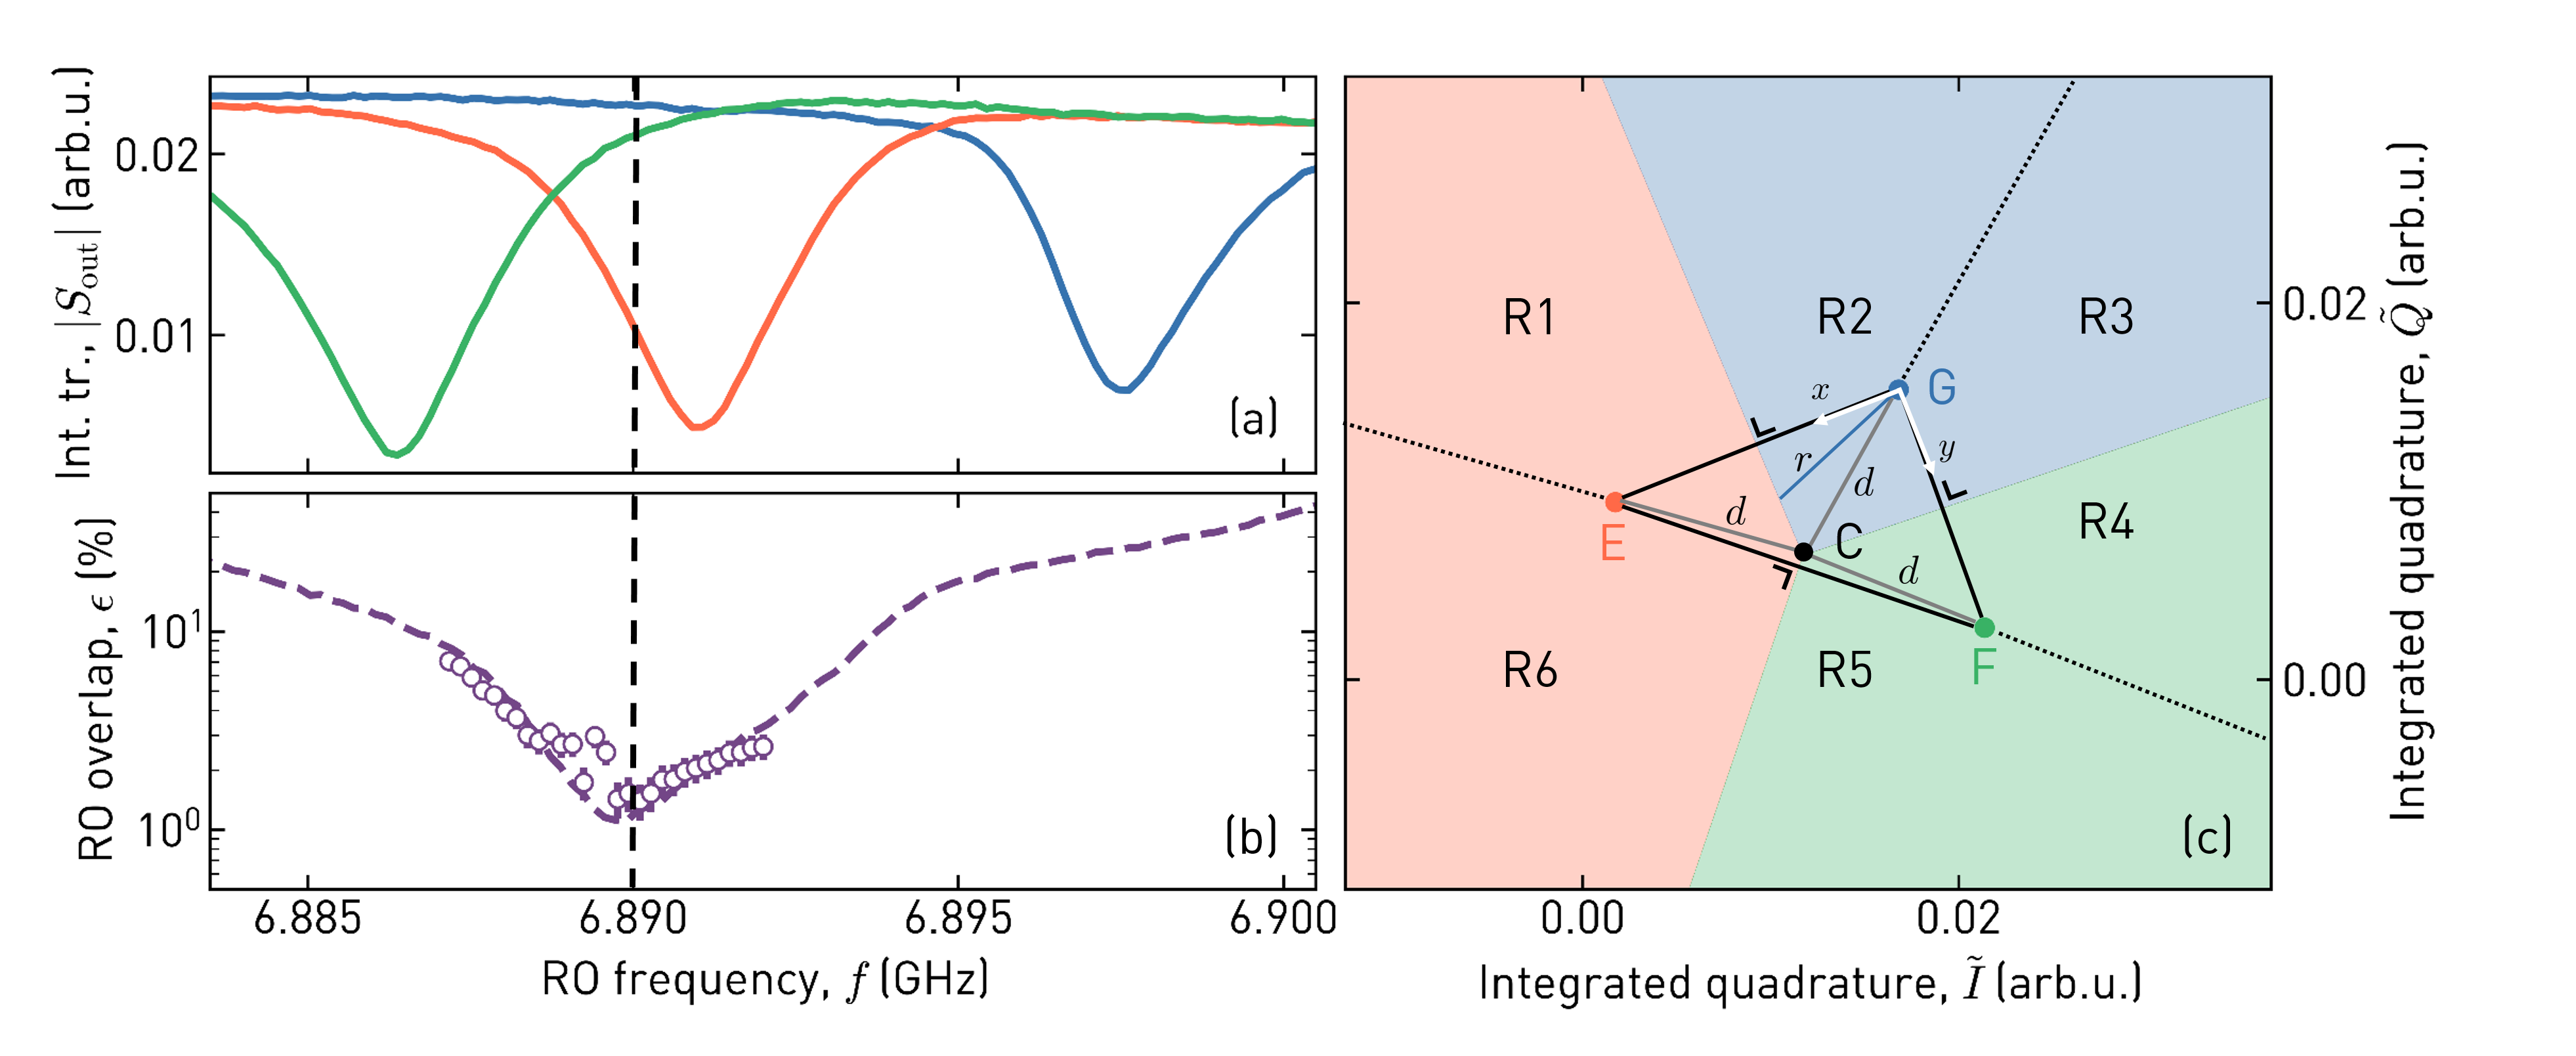
\includegraphics[width=\textwidth]{appendices/qutrit_readout/figs/ch3_readout_frequency_opt__with_iq_20200301_174851_ppt.png}
    \caption{Readout frequency optimization. (a) Amplitude of the integrated state-dependent resonator response (i.e. transmission) for qubit 2 prepared in \g{} (blue), \e{} (red), \f{} (green). (b) Average readout overlap (in \%) as predicted from the model (dashed line) and measured (scatter). (c). Integrated IQ-plane for $f = 6.890\unit{GHz}$ (dashed line in (a),(b)), the frequency for which the readout overlap is minimal. Points $G$, $E$, $F$ correspond to the average integrated resonator responds for states \g,\e{} and \f.  The shaded background color indicates which state is most likely according to a Gaussian mixture model with means centered in $G$, $E$ and $F$, and equal and isometric covariance. $R_i$ indicates different integration regions.  $C$ and $d$ indicate the circumcenter and circumradius respectively. }
    \label{fig:qutrit_readout_ro_freq_opt}
\end{figure}

In the case of equal and isometric covariance of the three distributions, for any measured data point, the distribution with the nearest mean (i.e. vertex of the triangle $GEF$) is the most likely distribution to have generated the data point. In addition, the decision boundaries coincide with the perpendicular bisectors of the triangle $GEF$\footnote{the perpendicular bisectors of a triangle are the collections of points for which the Eucledian distance to two vertices is equal.} (See Fig.~\ref{fig:qutrit_readout_ro_freq_opt}(c)).

Hence,  we compute the readout overlap $\epsilon_k$ consisting of the overlap between the 3 Gaussian distributions (one for each state) at each frequency $f_k$. The frequency yielding the smallest overlap between the Gaussian distributions results in highest \gls{snr} for all three states concurrently and is therefore chosen as readout frequency.

In the next section, we derive an analytical model to find the optimal readout frequency from the average time-integrated resonator responses and discuss the comparison between the model and experimental data shown in Fig.~\ref{fig:qutrit_readout_ro_freq_opt}(b).
 
\subsection{Analytical derivation} \label{s:analytical_derivation_3_gaussians}
We denote the state assignment probability matrix $A_k$ as function of the readout frequency $f_k$ and define the following variables,
\begin{itemize}
    \item[--] $ \mathcal{N}_i^{(k)}(\bm{x}|\bm{\mu}_i^{(k)}, \sigma^2\bm{I}) = \frac{1}{2\pi| \sigma^2\bm{I}|^{1/2}} \cdot \exp\left(-(\bm{x}-\bm{\mu}_i^{(k)})^T\, (\sigma^2\bm{I})^{-1}\,(\bm{x}-\bm{\mu}_i^{(k)})\right)$ the Gaussian distribution modeling measurement noise around state $s_i$ in the two-dimensional integrated IQ-plane at frequency $f_k$.
    \item[--] $\bm{\mu}_i^{(k)}$ the mean of the Gaussian distribution around state $s_i$ at frequency $f_k$, i.e. point $G$, $E$ and $F$ in Fig.~\ref{fig:qutrit_readout_ro_freq_opt}(c) for states \g, \e, \f{} at frequency $f_k = 6.890 \unit{GHz}$.
    \item[--] $\sigma^2\bm{I}$ the equal and isometric covariance of the Gaussian distribution.
    \item[--] $\bm{x}$ an arbitrary point $\in \R^2$ (for ease of notation, we translated the complex IQ-plane to a real, two-dimensional plane).
\end{itemize}

Based on Eq.~\eqref{eq:qutrit_readout_overlap}, the average readout overlap $\epsilon_{k}$ at frequency $f_k$ is, 
\begin{equation}
\epsilon_{k}= \frac{1}{3}\sum_{i=0}^{2}{\sum_{j \neq i}^{2}{P_k(s_j | s_i)}}
\end{equation}
where $P_k(s_j|s_i)$ is the probability of assigning a measurement to state $j$ while it was originally prepared as state $i$ at frequency $f_k$, with $j\neq i$. 

The minimization of the readout overlap is equivalent to a maximization of the trace of $A_k$ over all frequencies, such that finding the optimal readout frequency results in solving,
\begin{equation} \label{eq:opt_freq_proba}
f_{\mathrm{opt}} = \argmax_{f_k} \mathrm{Tr\left(A_k\right)} = \argmax_{f_k} \sum_{i=0}^2{P_k(s_i|s_i)}
\end{equation}

At each frequency, the probability $P(s_i|s_i)$ (we omit $k$ for clarity in the following equations) corresponds to the integral of the Gaussian density function $\mathcal{N}_i(\bm{x}|\bm{\mu}_i, \sigma^2\bm{I})$ over the domain where the density $i$ is higher than the density of any other state. Namely, the area of the two-dimensional IQ-plane in which an incoming point $\bm{x}$ will be correctly assigned $s_i$ if it was prepared in $s_i$. The integration domain are depicted in blue, red, green in Fig.~\ref{fig:qutrit_readout_ro_freq_opt}(c), for state \g, \e, and \f{} respectively.  The optimal readout frequency corresponds to the frequency yielding the largest sum of 3 similar integrals (one for each state)\footnote{For the readout of a two-level system, there are only two integrals and the approximation of equal and isometric covariance allows to ignore one more dimension using an appropriate rotation. The problem reduces to minimizing the overlap between two, one-dimensional Gaussian distributions, which is inversely proportional to the distance between the two means. Hence, the typical choice of readout frequency is the frequency yielding the largest difference between the two state responses~\cite{Heinsoo2018}.}. 

For ease of computation, each integration domain is further divided in 2 sub-domains. By symmetry, 
\begin{subequations}
\begin{equation}\label{eq:I1_integral}
    \int_{R1}{\mathcal{N}_0(\bm{x}|\bm{\mu}_0, \sigma^2\bm{I})\d\bm{x}} = \int_{R2} \mathcal{N}_2(\bm{x}|\bm{\mu}_2, \sigma^2\bm{I})\d\bm{x} = I_1 
\end{equation}
\begin{equation}
\int_{R3}{\mathcal{N}_2(\bm{x}|\bm{\mu}_2, \sigma^2\bm{I})\d\bm{x}} = \int_{R4} \mathcal{N}_0(\bm{x}|\bm{\mu}_0, \sigma^2\bm{I})\d\bm{x} = I_2 
\end{equation}
\begin{equation}
\int_{R5}{\mathcal{N}_2(\bm{x}|\bm{\mu}_2, \sigma^2\bm{I})\d\bm{x}} = \int_{R6} \mathcal{N}_1(\bm{x}|\bm{\mu}_1, \sigma^2\bm{I})\d\bm{x} = I_3 
\end{equation}
\end{subequations}
such that only 3 of the 6 sub-domain integrals need to be computed\footnote{ Note that additional weighting factor to the 3 integrals in this equation allow to favor \gls{snr} of 1 or 2 of the 3 states.},
\begin{equation}
\sum_{i=0}^2{P(s_i | s_i)} = 2 \cdot ( I_1 + I_2 + I_3) \label{eq:total_non_overlap}
\end{equation}

We provide a detailed derivation for $I_1$. The other two integrals are solved in the similar way but are preceded by an appropriate rotation and translation of the coordinate system. 

We start by a shift of coordinate system with the origin at point $G$ and the x-axis aligned with the line segment $|GE|$ such that $\mu_0 = 0$ (see white coordinate system in Fig.~\ref{fig:qutrit_readout_ro_freq_opt}(c)), followed by a polar coordinate transformation. In this parametrization, the radius of integration $r$ is a function of $\theta$, the angle between the x-axis of the coordinate system centered in point $G$ and $r$. Namely,
\begin{equation}
r(\theta) =\begin{cases}
    m / \cos \theta, & \text{if $-\pi/2<\theta<\pi/2$}.\\
    +\infty, & \text{otherwise}.
  \end{cases} 
\end{equation} 
with $m$ being the distance between $G$ and the midpoint of ($G$, $E$), and assuming $\theta \in [-\pi, \pi[$. The integration bounds of $\theta$ are $ \pi - \gamma$ and $\gamma$ where $\gamma = \arccos{d/m}$.

Eq.~\eqref{eq:I1_integral} becomes in the new coordinate system
\begin{equation}
I_1 = \int_{R2} \frac{1}{2\pi \sigma^2} e^{-\frac{\bm{x}^\intercal \bm{x}}{2 \sigma^2}} \d\bm{x}
\end{equation}
and in polar coordinates with the corresponding integration boundaries, 
\begin{equation}\label{eq:qutrit_integral_polar}
I_1=\begin{cases}
    \int_{\gamma - \pi}^{\gamma}\int_0^{m/\cos \theta}{\frac{1}{2\pi \sigma^2} \exp{\left(-\frac{\rho^2}{2 \sigma^2}\right)}\, \rho \,\d\rho \,\d\theta}, & \text{if $-\pi/2<\theta<\pi/2$}.\\
    \int_{\gamma - \pi}^{\gamma}\int_0^{\infty}{\frac{1}{2\pi \sigma^2} \exp{\left(-\frac{\rho^2}{2 \sigma^2}\right)}\,\rho \,\d\rho \,\d\theta}, & \text{otherwise}.
  \end{cases}
\end{equation}
We note that the inner integral in both cases is the derivative of a Gaussian (up to a constant),
\begin{equation}
\int_0^{a}{\frac{1}{2\pi \sigma^2} \exp{(-\frac{\rho^2}{2 \sigma^2})}\rho \,\d\rho \,\d\theta} =\frac{1}{2\pi} \left(1 - \exp{\left(\frac{-a^2}{2\sigma^2}\right)}\right)
\end{equation}
and therefore simplify Eq.~\eqref{eq:qutrit_integral_polar} to
\begin{equation}
I_1 =
\begin{cases}
    \int_{\gamma - \pi}^{\gamma}{\frac{1}{2\pi} \left(1 - e^{-\frac{m^2}{2 \sigma^2 \cdot \cos^2{\theta}}}\right)\,\d\theta}, & \text{if $-\pi/2<\theta<\pi/2$}.\\
    \int_{\gamma - \pi}^{\gamma}{\frac{1}{2\pi}\d\theta}, & \text{otherwise}.
  \end{cases}
\end{equation}

Since $\int_{\gamma - \pi}^{\gamma}{\frac{1}{2\pi}\d\theta}$ is independent of both $\theta$, it results in a constant function integrated over $\pi$. This simplifies $I_1$ further,
\begin{equation} \label{eq:final_frequency_I_integral}
    I_1 = \frac{1}{2} - 
    \begin{cases}
    \int_{\gamma - \pi}^{\gamma}{e^{-\frac{m^2}{2 \sigma^2 \cdot \cos^2{\theta}}}\,\d\theta}, & \text{if $-\pi/2<\theta<\pi/2$}.\\
    0, & \text{otherwise}.
  \end{cases}
\end{equation}
The 0 values for $\theta$ prevent the remaining integral to have a closed form solution, but it can easily be computed numerically. 

An analogous development holds for $I_2$ and $I_3$ for each frequency, the average overlap yields,
\begin{equation} \label{eq:qutrit_ro_overlap_from_integral}
    \epsilon_k = 1 - \frac{2}{3}\cdot \sum_{i=1}^{3}{I_{i,k}}
\end{equation}
and the optimal readout frequency is extracted as defined in Eq.~\eqref{eq:opt_freq_proba},
\begin{equation} \label{eq:optimal_freq}
    f_{\mathrm{opt}} = \argmax_{f_k} {\sum_{i=1}^{3}{I_{i,k}}}
\end{equation}

In Fig.~\ref{fig:qutrit_readout_ro_freq_opt}(b), we show the readout overlap $\varepsilon = \epsilon\cdot 100\%$ computed with Eq.~\eqref{eq:qutrit_ro_overlap_from_integral} for the integrated resonator responses of Fig.~\ref{fig:qutrit_readout_ro_freq_opt}(a) with a dashed, purple line. The minimum average overlap is $~1\unit{\%}$ at $f_{\mathrm{opt}} = 6.890\unit{GHz}$ (dashed black line). 

\subsection{Comparison to experimental data}
We validate the model by experimentally sweeping the readout frequency, recording 20000 single-shot measurements for each eigenstate, and assigning the shots to reconstruct $A_k$ near the frequency of interest. The total (average) experimental error is $1-\mathrm{Tr}\left(A_k\right)/3$. However, the latter includes not only readout overlap errors, but also errors originating from \t{1}-decay and thermal population. Therefore, we use preselection on the single-shot measurements to mitigate the effect of thermal population (see Appendix \ref{app:setup}). To account for errors expected from \t{1}-decay for levels \e{} and \f, we subtract $1-\exp{\left(-t/T_1^{ge}\right)}/3$ and $1-\exp{\left(-t/T_1^{ef}\right)}/3$ from the total error, where $t$ is half the readout length (200 ns). We use $T_1^{ge} = 27.7\, \mu s$ which we measured prior to the single-shot measurements and thereby also infer $T_1^{ef} \approx 27.7 / \sqrt{2}\, \mu s$. The estimated readout overlap errors, which we show in scattered points in Fig.~\ref{fig:qutrit_readout_ro_freq_opt}(b), are in good agreement with the model.

To further reduce the errors caused by readout overlap, we describe in the next section the choice of mode-matched integration weights that linearly increase the \gls{snr}. Note that, since the integration is linear, the readout frequency found in this section remains optimal with mode-matched integration weights.

\section{Mode-matched integration weights} \label{s:mode_matched_integration}
With the readout frequency fixed, we define the mode-matched integration weights for single-shot readout. In a two-level system, taking the complex conjugate of the difference between the average ground and excited state responses of the readout pulse as mode-matched filter coefficients is shown to provide near-optimal filter efficiency~\cite{Heinsoo2018, Gambetta2007, Bultink2018}. The mode-matched weighted integration of the time trace $S_{\mathrm{out}}(t)$ is then: 
\begin{equation}
    x_1 = \int_{0}^{T}{w_{1}(t)\cdot S_{\mathrm{out}}(t)\d t} 
\end{equation}
where $w_{1}(t)$ are the mode-matched weights described above. The index specifies that this is the complex weights corresponding to the \textit{first} integration unit.
A second integration unit is defined to extend this scheme to a three-level system~\cite{Reuer2018}. More specifically, the second integration unit and corresponding weights, $w_2(t)$, are chosen such that $\{w_{1}(t), w_{2}(t)\}$ is a basis spanning the hyper-plane defined by the average response of the three states. Similarly to the two-level case, $w_{2}(t)$ corresponds to the complex conjugate of the difference between the average ground and \textit{second} excited state responses.

These two sets of complex weights are then uploaded on the \gls{uhf} to perform real-time integration of the time traces, such that each single-shot measurement results in a two-dimensional data point (one for each integration unit), $\bm{x}$, where the integral is replaced by a sum,
\begin{equation}
        x_i = \sum_{t=0}^{T}{w_{i,t}\cdot S_\mathrm{out, t}} \text{ for $i \in \{1,2\}$}
\end{equation}
and the time interval is the sampling rate of the \gls{uhf} (2.4\unit{GHz}).

\section{Characterization of three-level single-shot readout} \label{s:experimental_data}
Three-level single-shot readout has been previously been demonstrated on transmon qutrits~\cite{Kurpiers2018DeterministicPhotons, Magnard2018FastQubit}. This section demonstrates the ability to perform single-shot readout on a transmon with a correct state assignment probability of 98.52\%\footnote{For the comparison between three-level and two-level readout performance on the same qubit, see~\cite{Lacroix2019}.}. To the best of our knowledge, this exceeds other correct state assignment probabilities reported in literature for transmon qutrits. In addition, we describe how to use the readout scheme to characterize the three-level populations in any measurements and illustrate it on the  $T_1$ measurement of the \f-level.

\subsection{Single-shot readout characterization} \label{sec:qutrit_readout_ro_characterization}
We use the following calibration routine to assess the performance of the qutrit readout:
\begin{enumerate}
    \item Calibrate parameters of the $R^{\pi}_x$ rotation pulse to prepare the qubit in state $|e\rangle$. 
    \item Calibrate parameters of the second excitation pulse to prepare the qubit in state $|f\rangle$.
    \item Measure average, time-dependent readout responses of the resonator for each eigenstate with the readout pulse frequency $f_{\mathrm{opt}}$ obtained as described in Section \ref{s:frequency_optimization}. The complex conjugate difference in IQ-plane between the ground and first excited state time-traces is taken as integration weights for the first integration unit. The second is defined by using the Gram-Schmidt algorithm~\cite{Bjorck1994NumericsOrthogonalization} on the complex conjugate difference between the ground and second excited state to find an vector, ortho-normal to the first set of integration weights, and spanning the hyperspace of the 3 eigenstates. 
    \item Upload the two sets of integration weights,  $\{w_1, w_2\}$, to the \gls{uhf} for real-time integration.
    \item Prepare each eigenstate 50000 times\footnote{Empirically found to be a  number of shots achieving low statistical estimation errors.}, which after real-time integration results in a two-dimensional data point per shot.
    \item Fit a \gls{gmm} to the dataset of integrated shots using the expectation maximization algorithm~\cite[p.~434-439]{Bishop2006} with the constraint of equal covariance. 
    \item Assess the readout by constructing the state assignment probability matrix.
\end{enumerate}

We apply this procedure to qubit 1 of the device described in Appendix \ref{app:setup} and present the results in Fig.~\ref{fig:ssro_opt}. The corresponding mode-matched integration weights, as well as the readout parameters optimization are reported in~\cite[Appendix B]{Lacroix2019}.

Predicting the most likely state on the entire 2D-plane results in the decision boundaries indicated by the background color of the experimental data in Fig.~\ref{fig:ssro_opt}(a). These one-dimensional boundaries can be interpreted as the natural extension of the threshold (zero-dimensional) used in a two-level system for assigning a shot to the ground or excited state. 

\begin{figure}[t]
  \centering
    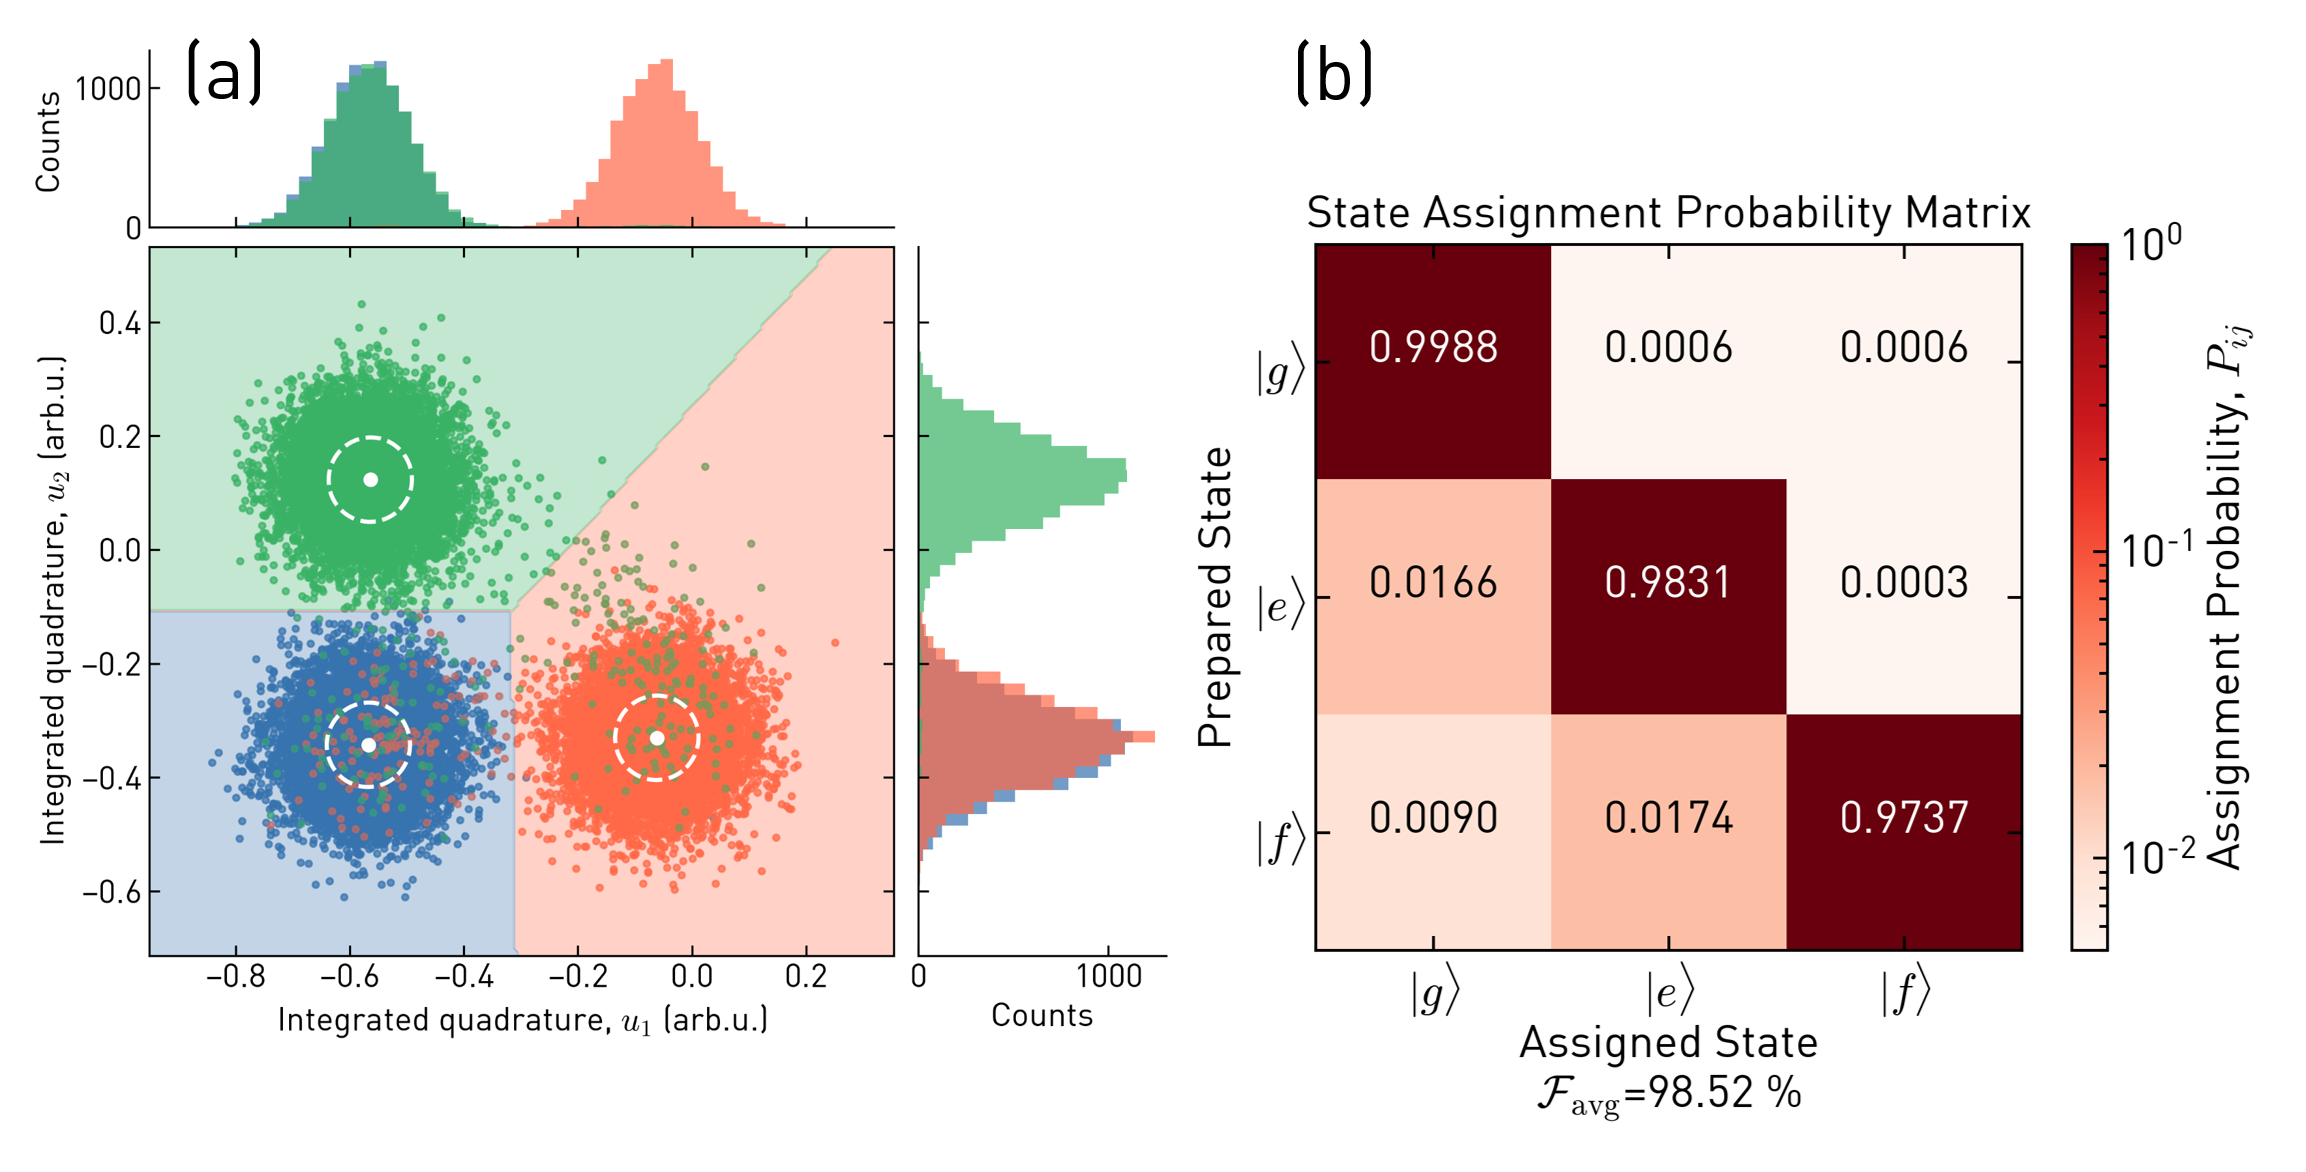
\includegraphics[width=\textwidth]{appendices/qutrit_readout/figs/ch3_readout_GMM_scatter_and_hist_20200116_144401_combined.png}
   \caption{Statistically optimal state assignment with mode-matched integration weights. (a) First 10000 of 50000 single-shot measurements for each eigenstate preparation of qubit 1. Preselection was performed to mitigate thermal population (see Appendix \ref{app:setup} for thermal population estimates). The boundaries correspond to the decision boundaries of the fitted \gls{gmm}. The white points correspond to the position of the means of each Gaussian component and the circle to the standard deviation. In addition, marginal histogram distributions are displayed right and above the main plot. (b) State assignment probability matrix corresponding to the 3x50000 single-shot measurements presented in (a), after pre-selection. The rows correspond to the prepared states and the columns to which state the prepared eigenstates were assigned using the \gls{gmm}.}
  \label{fig:ssro_opt}
\end{figure}

We show the corresponding state assignment probability matrix, $A$, in Fig.~\ref{fig:ssro_opt}(b). The average three-level correct state assignment probability is defined as
\begin{equation}
    \mathcal{F}_{avg} = \frac{1}{3}\mathrm{Tr}(A)
\end{equation}
For the presented run, it amounts to 98.52\%. Notable observations for each matrix row:
\begin{itemize}
    \item $|g\rangle$: Preselection procedure removes the majority of the thermal population (on the order of 1\%, see Appendix \ref{app:setup}). We estimate 0.05\% measurement-induced transition by counting the number of ground-state data points further than 5 standard deviations away from the mean\footnote{Decision boundaries are approximately 3.3 standard deviations away from the mean. The probability that an error is caused by readout overlap is much smaller than by measurement-induced excitation at a distance of 5 standard deviation from the mean.}. remaining errors are caused by the overlap between the distributions.
    \item $|e\rangle$: 
    \begin{itemize}
        \item The assignment of a $|g\rangle$ state for a $|e\rangle$ preparation is dominated by $T_1$-decay. Given a $T_1$ of $25.11\, \mu s$ (last recorded $T_1$) 1.11\% of the prepared $|e\rangle$ shots decay during the first 280\unit{ns} of the readout\footnote{The entire readout is 400\unit{ns} long but only decay events before the first 280\unit{ns} are expected to be misclassified. This corresponds to the time at which 50\% of the information (i.e. integral of the absolute value of mode-matched weights) to distinguish \g{} and \e{} is acquired}. This number explains an important fraction of the observed 1.66\%. 
        The overlap of distributions due to finite \gls{snr} is another source of errors.
        \item The assignment of $|f\rangle$ state for a $|e\rangle$ likely arise from measurement induced transitions, amounting to approximately 0.02\%. Errors originating from readout overlap errors likely explain other errors. 
    \end{itemize}
    \item $|f\rangle$: similarly, misclassification of the $|f\rangle$ state is dominated by $T_1^{ef}$ decay. With a $T_1^{ef}$ of $\sim14.4\, \mu s$,  1.93\% of the initial \f{} population are expected to decay to \e{} or \g. The largest fraction thereof is expected to be classified as $|e\rangle$, while a smaller fraction is expected to have decayed twice during the measurement. The remaining 0.7\% are partially explained by readout overlap errors and preparation errors (which are expected to be higher than \e-level preparation errors because the \f-level preparation requires two pulses).
\end{itemize}

These numbers are summarized in Table \ref{tab:error_mechanisms}. Overall, the error mechanism dominating the state assignment probability matrix is $T_1$- and $T_1^{ef}$-decays, which explain on average 1.01\% of the 1.48\% errors. The total readout overlap error of the Gaussian components, computed using the method described in  \ref{s:analytical_derivation_3_gaussians}, amounts to 0.072\%. Estimated measurement-induced transitions explain on average 0.07\%. Remaining errors amount to 0.33\%, which we suspect are related to fluctuations in $T_1$ and $T_1^{ef}$ as measurement-induced transitions are extremely small on this qubit. This analysis also does not take into account errors originating from leakage into the $\ket{h}$ (or higher) state(s). These errors can lead to misinterpretation of misclassifications of the \f-level in the observed subspace of states $\{\ket{g}, \ket{e}, \ket{f}\}$, depending on where those higher states are projected in the integrated plane. We do observe such effects when optimizing the readout amplitude (see~\cite[Appendix B, Fig.~11]{Lacroix2019}). However, even if not completely negligible, these errors do not impact directly the subspace of interest spanned by $\{\ket{g}, \ket{e}\}$. Indeed, they mostly occur due to measurement-induced transitions on prepared \f-states, which we do not use directly when running quantum algorithms in the computational subspace. 

\begin{table}[ht]
\centering
\caption{Error mechanisms for the measurement displayed in Fig.~\ref{fig:ssro_opt}.}
\begin{tabularx}{0.65\textwidth}{ll}
\toprule 
\textbf{Error mechanism} & \textbf{Error (\%)} \\
\midrule
    $T_1$ and $T_1^{ef}$-decay & 1.01 \\
    Readout overlap & 0.07\\
    Measurement-induced transitions &  0.07 \\
    \midrule
    Total explained errors & 1.15  \\
    \midrule
    Total errors & 1.48 \\
\bottomrule
\end{tabularx}
\label{tab:error_mechanisms}
\end{table}

This analysis suggests that improving the qubits lifetime and/or increasing the readout speed is the most effective way to further increase the correct state assignment probability. In cases where the overlap errors are higher, it might be worth exploring  bi-chromatic readout pulses~\cite{Collodo2020}. Indeed, this method could help increasing the \gls{snr} between the 3 eigenstates, thereby reducing overlap errors. It could also help reducing the readout amplitude, which in turn can contribute reducing measurement-induced leakage. It remains unclear whether the improvements this readout pulse may provide are significant and worth the overhead of calibrating additional parameters.

In summary, we have demonstrated the ability to perform three-level, single-shot readout with an average correct assignment probability superior to 98\% on a transmon qutrit. The assignment errors are dominated by decay events during the 400\unit{ns} readout  originating from the finite lifetime of the \e{} and the \f{} level. In the next section, we detail how to monitor the populations of the first three basis states of a transmon with this readout scheme for arbitrary measurements and illustrate the scheme on a \t{1}-measurement of the \f{} level.

\subsection{Using the three-level readout} \label{sec:qutrit_readout_correction}
After calibration on reference single-shot readout measurements, the \gls{gmm} enables the assignment of state labels to single-shots in any measurement. The fraction of single-shot assigned to each of the state \g, \e{} and \f{} yield (measured) estimates $\bm{P}^m = (P_g^m, P_e^m, P_f^m)^\intercal$ for the populations $\bm{P} = (P_g, P_e, P_f)^\intercal$ of Eq.~\eqref{eq:qutrit_state}~\cite{Magnard2018FastQubit}.

However, as discussed in Section \ref{sec:qutrit_readout_ro_characterization}, the state assignment is sensitive to readout imperfections and therefore yields biased population estimates. For instance, a pure \e{} state measurement should result in $\bm{P}^m = (0,1,0)^\intercal$ but might instead yields $\bm{P}^m = (0.017,0.983,0.0)^\intercal$, just as in the calibration measurement. To account for these imperfections, we use a latent variable model~\cite{Cai2012LatentModeling} to infer the (corrected) qutrit populations $\bm{P}^c$ relative to the calibration measurement,
\begin{equation}
    A^\intercal \cdot \bm{P}^c = \bm{P}^m
\end{equation}
where $\bm{P}^c$ are the latent (corrected) qutrit populations (3x1), $\bm{P}^m$ are the measured qutrit populations and $A$ is the reference state assignment matrix obtained during calibration. To infer $\bm{P}^c$, we multiply the measured population by the transpose inverse of the reference state assignment probability matrix,
\begin{equation} \label{eq:mtx_inversion}
     \bm{P}^c = (A^{\intercal})^{-1} \cdot\bm{P}^m
\end{equation}
where $(A^{\intercal})^{-1}$ can be seen as a linear filter acting on $\bm{P}^m$. 

Note that this procedure assumes that $A$ stays constant over time, which is not evidently fulfilled. For instances, fluctuations in $T_1^{ge}$ and $T_1^{ef}$ directly induce fluctuations in $A$, which can lead to over- or under-correction of the populations. Therefore, a reference matrix $A$ must be recorded at the end of each measurement sequence, similarly to \g{} and \e{} state calibration points typically used in Rabi oscillation measurements. 

In Fig.~\ref{fig:t1ef_3lv}, we display the time evolution of the measured qutrit populations for a $T_1$-measurement of the \f-level. The scattered points, which correspond to the measured populations $\bm{P}^m$, are in excellent agreement with the rate-equation evolution shown in solid lines. The rate-equation accounts for thermal population and its only free the parameter is $T_1^{ef}$, for which we find a value of $14.96 \pm 0.09 \,\mu\textrm{s}$. 

At short time scales, the qutrit is in the second excited state and progressively decays into the first excited state. $P_e^m$ first grows exponentially as $P_f^m$ decays with the time constant of T$_1^{ef}$. After approximately 20 $\mu s$, the decay from the \e-state to the \g-state with time constant T$_1^{ge}$ becomes more important than the remaining incoming population from the \f-level.  This results in a decrease of the \e-level population at larger time scales. The \g-state population is zero at the start of the measurement and increases progressively as the time evolving population of the \e-level decays into the \g-state. The population dynamics in this measurement illustrate that obtaining a good estimate for $T_1^{ef}$ is more intricate without three-level readout because there is no way easy way to detect the cascaded decay without monitoring all states. 

% The readout procedure also provides an accurate estimate of the leakage in the \f-level for operations which are meant to stay in the computational space, such as two qubit gates. The precise monitoring of leakage during two qubit gates calibration ensure the chosen pulse parameters do not result in leakage. 

% As the number of qubits on quantum processors grows, the speed of the calibration also becomes a

\begin{figure}[ht]
  \centering
     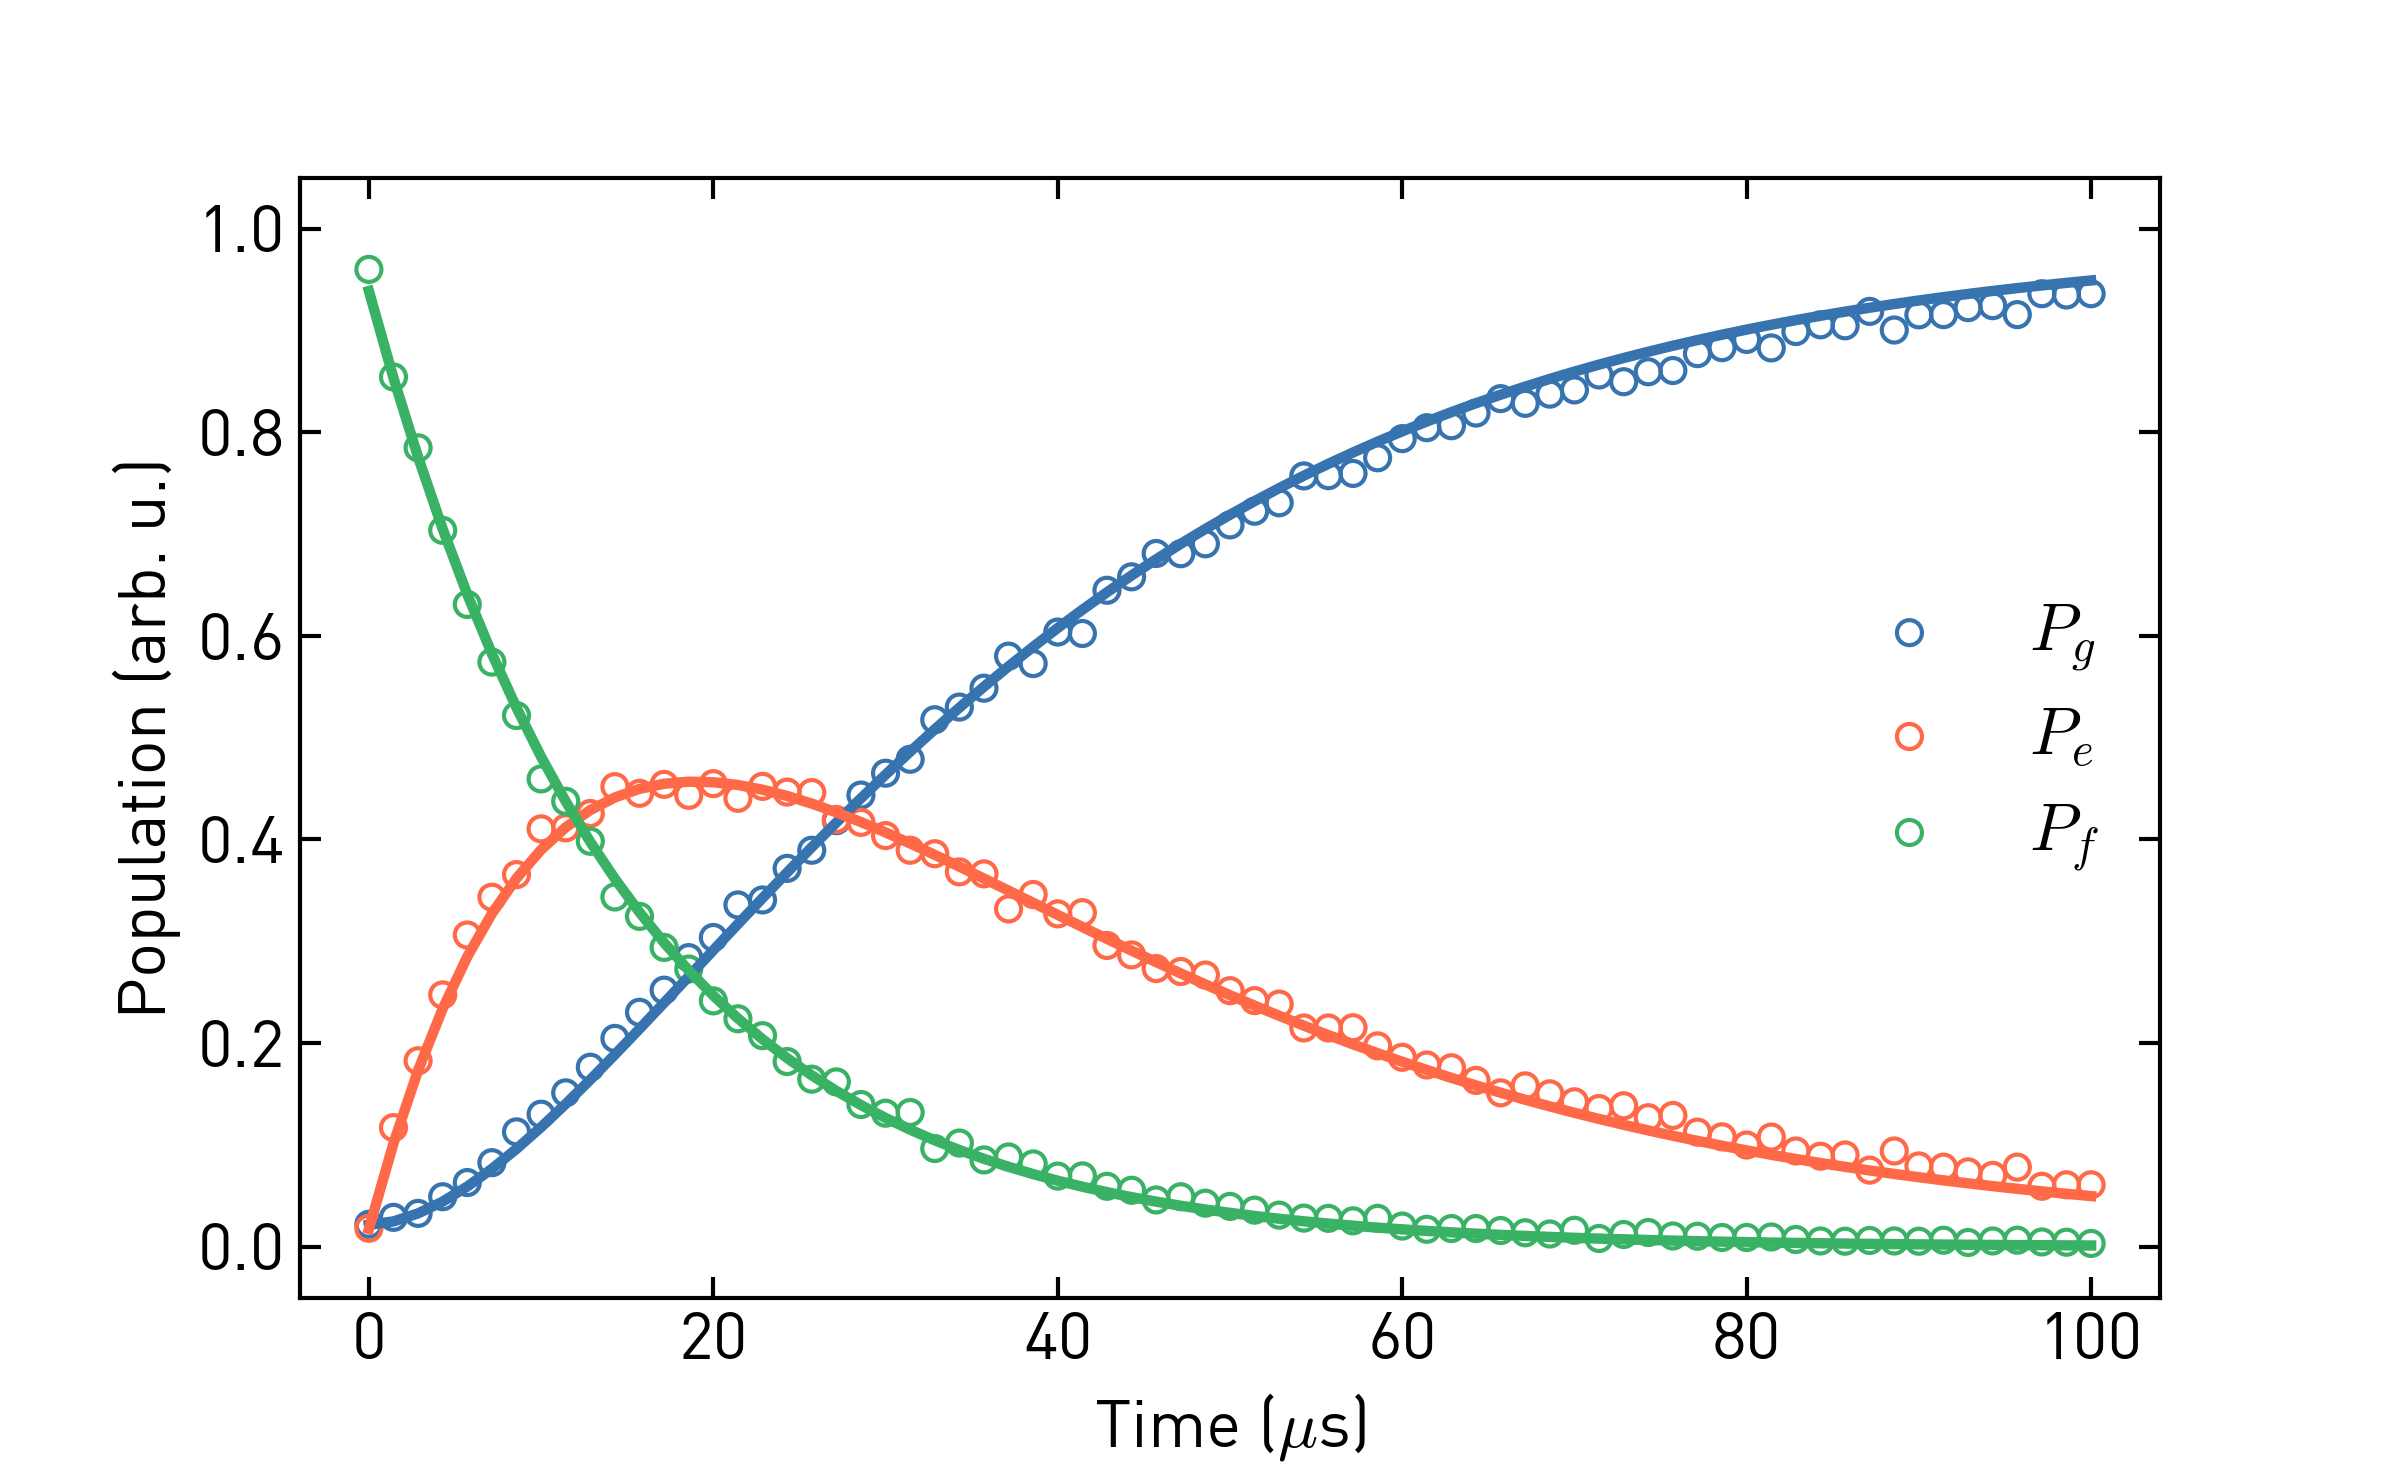
\includegraphics[width=\textwidth]{appendices/qutrit_readout/figs/readout_t1ef_20200302_004024.png}
\caption{Illustration measurements of the three-level readout scheme on qubit 1.  $T_1$ measurement of the \f-level. Time evolution of measured population for each eigenstate (scattered) and population extracted from a rate-equation (solid lines) that accounting for thermal population. We extract a \f-level lifetime of $14.96\, \mu \textrm{s}$.}
\label{fig:t1ef_3lv}
\end{figure}

In the next section, we describe another application of the three-level readout scheme, namely the active reset of a qutrit to its ground state. 

\section{Three-level, measurement-based active reset} \label{sec:active_reset}
Low-latency analysis of quantum states is key for many quantum algorithms, including quantum error correction~\cite{Reed2012RealizationCircuits}, quantum teleportation~\cite{Steffen2013DeterministicSystem}, quantum deep learning~\cite{Cao2017QuantumComputers} and active qubit reset~\cite{Magnard2018FastQubit, Salathe2018Low-LatencyCommunicationb}. These algorithms employ the (assigned) projected state to condition further operations in the quantum circuit. To ensure success of the algorithm, the analysis and feedback operation must occur much faster than the coherence time of the system. 

In this section, we adapt the three-level readout introduced in Section~\ref{s:high_level_description} to perform low-latency state assignment as required for feedback experiments. Next, we use the three-level state assignment in a feedback loop with a transmon to actively reset a qutrit to its ground state. 

\subsection{Setup and procedure for low-latency analysis of quantum states}
We show simplified schematics of our experimental setup in Fig.~\ref{fig:readout_active_reset_schematics}(a) (see Appendix~\ref{app:setup} for detailed schematics). We use Zurich Instruments' \gls{uhf} for readout combined with Zurich Instruments' \gls{hdawg} for drive and feedback pulses generation.

\begin{figure}
    \centering
    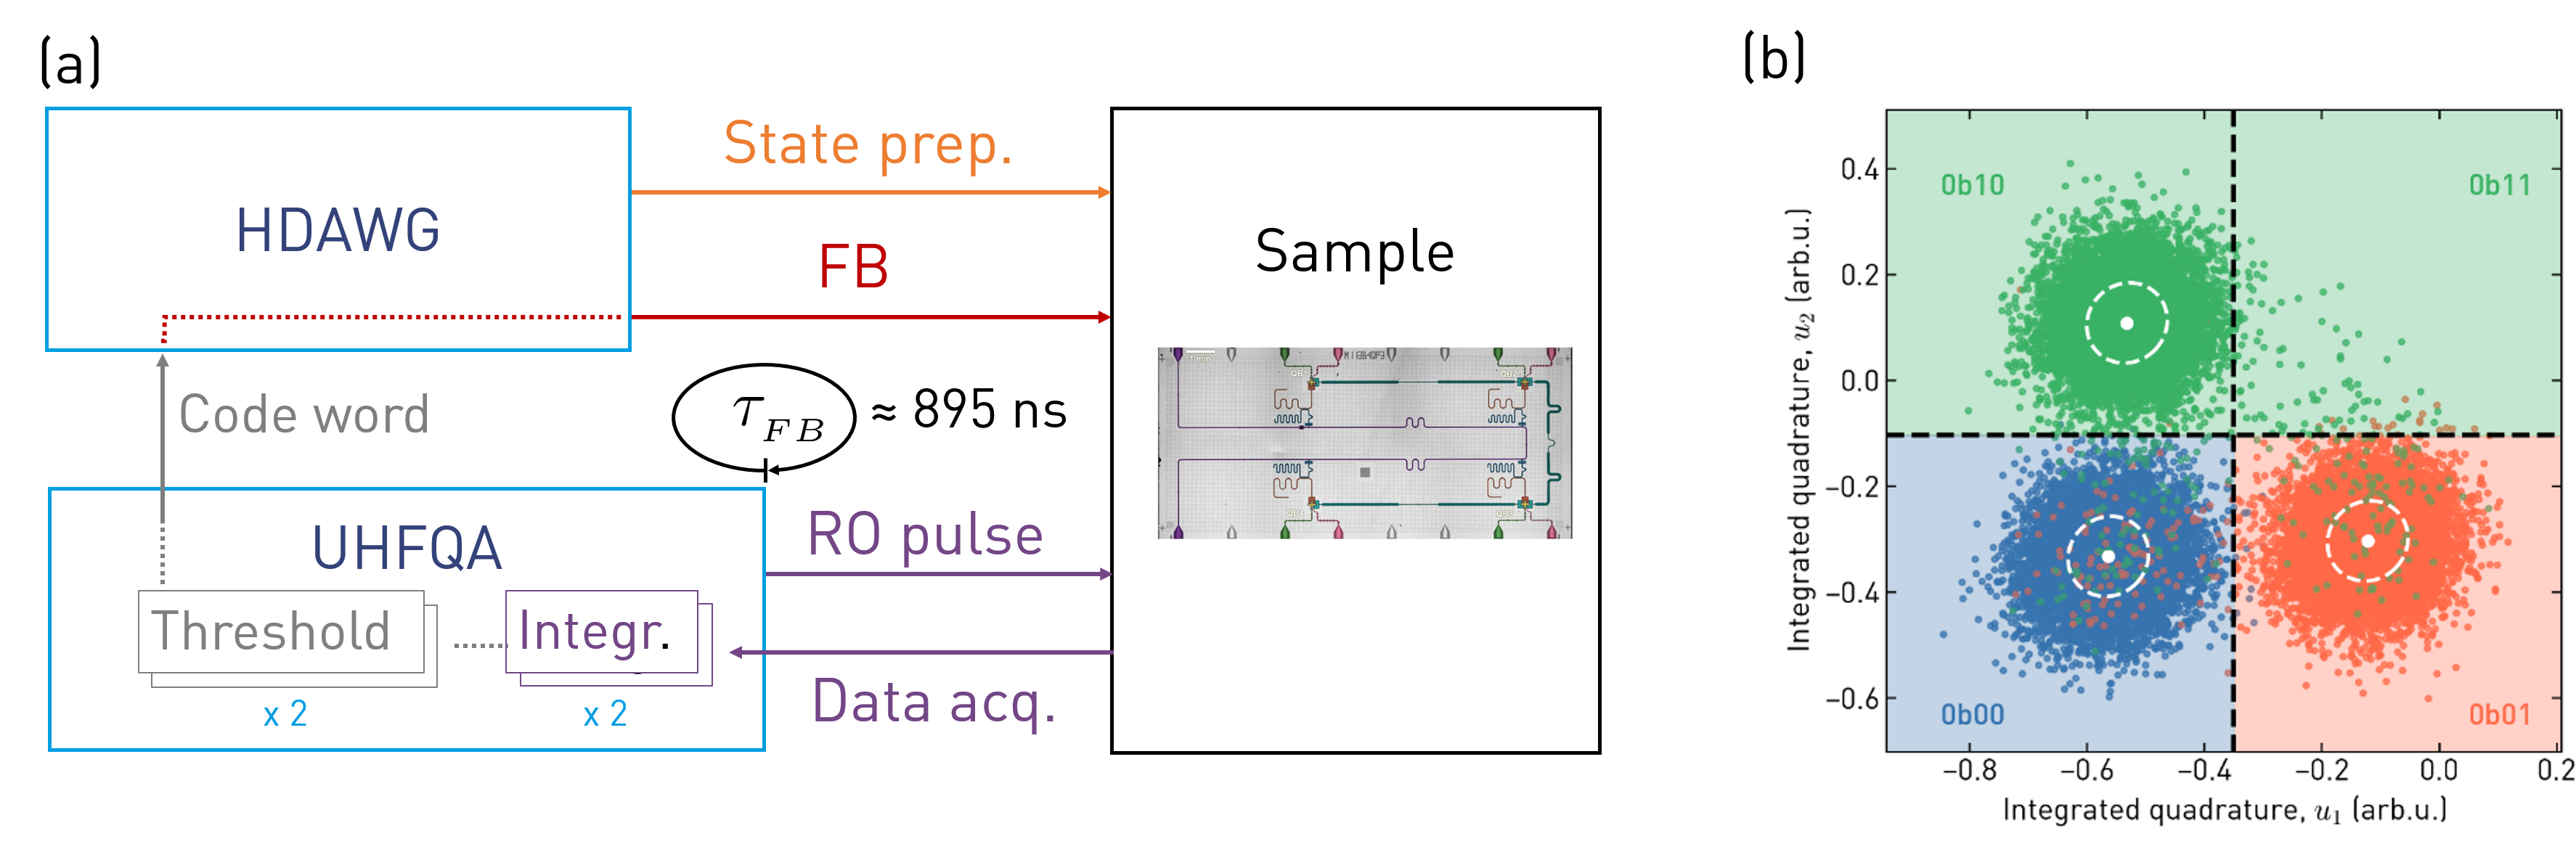
\includegraphics[width=\textwidth]{appendices/qutrit_readout/figs/ch3_readout_active_reset_setup.png}
    \caption{(a) Simplified schematics of the experimental setup: the \gls{hdawg} is used for pulse generation and the \gls{uhf} for readout pulse generation, data acquisition, integration, state assignment, and code word generation. (b) Calibration measurement of the three-level, single-shot readout on qubit 1 to determine the threshold required by the \gls{uhf} for real-time state assignment. The two thresholds are indicated with black, dashed lines. The background color corresponds to the state associated with the code word for each region. The corresponding code words for each regions are displayed in the corners. Blue, red, green correspond to states \g, \e and \f{} respectively. The white dot and circle correspond to the mean and standard deviations of each distribution.}
    \label{fig:readout_active_reset_schematics}
\end{figure}{}

A feedback experiment typically consists of four steps: state preparation, readout, state assignment and feedback operation(s). First, we send microwave pulses generated by the \gls{hdawg} to prepare the quantum state. Next, we send a readout pulse and record the transmission line response with the \gls{uhf}. As described in Section \ref{s:mode_matched_integration}, we integrate\footnote{The \gls{uhf} includes a field programmable gate array (FPGA) that integrates the response in real-time.} the response with mode-matched integration weights yielding a two-dimensional data point for each single-shot measurement. We assign the point to a state in about 400\unit{ns} with predefined thresholds on each integration unit axis, as pictured in Fig.~\ref{fig:readout_active_reset_schematics}(b). We use a decision tree classifier~\cite{Breiman1984} of depth 2 fitted with the CART algorithm~\cite{Breiman1984} to find thresholds on each axis that minimizes the Gini impurity~\cite{Bishop2006, Breiman1984}. In the limit of average \gls{snr} larger than 7, the expected difference in average correct state assignment probability between decision tree classifier and a \gls{gmm} is on the order of $1\permil$ (see~\cite{Lacroix2019} for more details about when this comparison is valid). For the instance presented in Fig.~\ref{fig:readout_active_reset_schematics}(b), the decision tree classifier in fact outperforms the \gls{gmm} by $1\permil$ because it exploits the non-Gaussian distribution of decaying events.
The \gls{uhf} generates binary a two-bit code word (one for each integration channel) defining the location of the data point: the bit is zero if the data point is smaller than the threshold on that axis and 1 if it is larger. The code word is sent over a digital input/output (DIO) port to the \gls{hdawg} that sends different pulses to the device depending on the code word value.

\subsection{Demonstration of three-level active reset}
We use this experimental framework to actively reset a qutrit to its ground state. We characterize the reset procedure for a qutrit prepared in each of the three eigen states with the pulse scheme presented in Fig.~\ref{fig:readout_active_reset_schematics}(a). We prepare the qutrit in \g, \e, or \f{} and then perform $N$ cycles of readout, state assignment and feedback pulses. For each cycle, no pulse is sent to the qutrit if the assigned state is \g. By contrast, if the assigned state is \e{} (\f), single qutrit control pulse(s) $R_{ge}^{\pi}$ ($R_{ef}^{\pi}$ and subsequently $R_{ge}^{\pi}$) are employed to bring the qutrit back to \g. We perform a last readout after the $N$ cycles to characterize the effect of the last feedback pulse.

Each cycle takes approximately 895\unit{ns}; 350\unit{ns} for the readout, 440\unit{ns} for state assignment, code word generation and logical branching in the \gls{hdawg}, 100\unit{ns} to apply the feedback operations  and 5\unit{ns} buffer before the next readout. We fix the time-window reserved for the feedback operations to 100\unit{ns} (which corresponds to the longest possible feedback sequence: two, 50\unit{ns} long single qutrit gates) independently of the assigned state because the state is known only at run time but all triggers are compiled before the start of the measurement.

We present the evolution of the readout-corrected populations $P_{g,e,f}^c$ over time after state preparation in  Fig.~\ref{fig:qutrit_readout_active_reset_populations}(b)-(d).
For reference, we perform the exact same measurement without reset pulses and display the corresponding populations $P_{g,e,f}^{NR}$ with translucent colors. We define the excited state population, $P_\textrm{exc} = 1 - P_g$ and indicate with a red dashed-line the average, steady-state excited population when no reset is applied,
\begin{equation}
    \langle P_{\textrm{exc, ss}}^{NR}\rangle = \frac{1}{N+1}\sum_{n=0}^{N} 1-P_{\textrm{exc},n}^{NR}
\end{equation}
where $P_{\textrm{exc},n}^{NR}$ is the excited state population at the $n$-th readout for a qutrit prepared in \g{}, and $N+1$ is the total number of readouts.

\begin{figure}[ht]
    \centering
    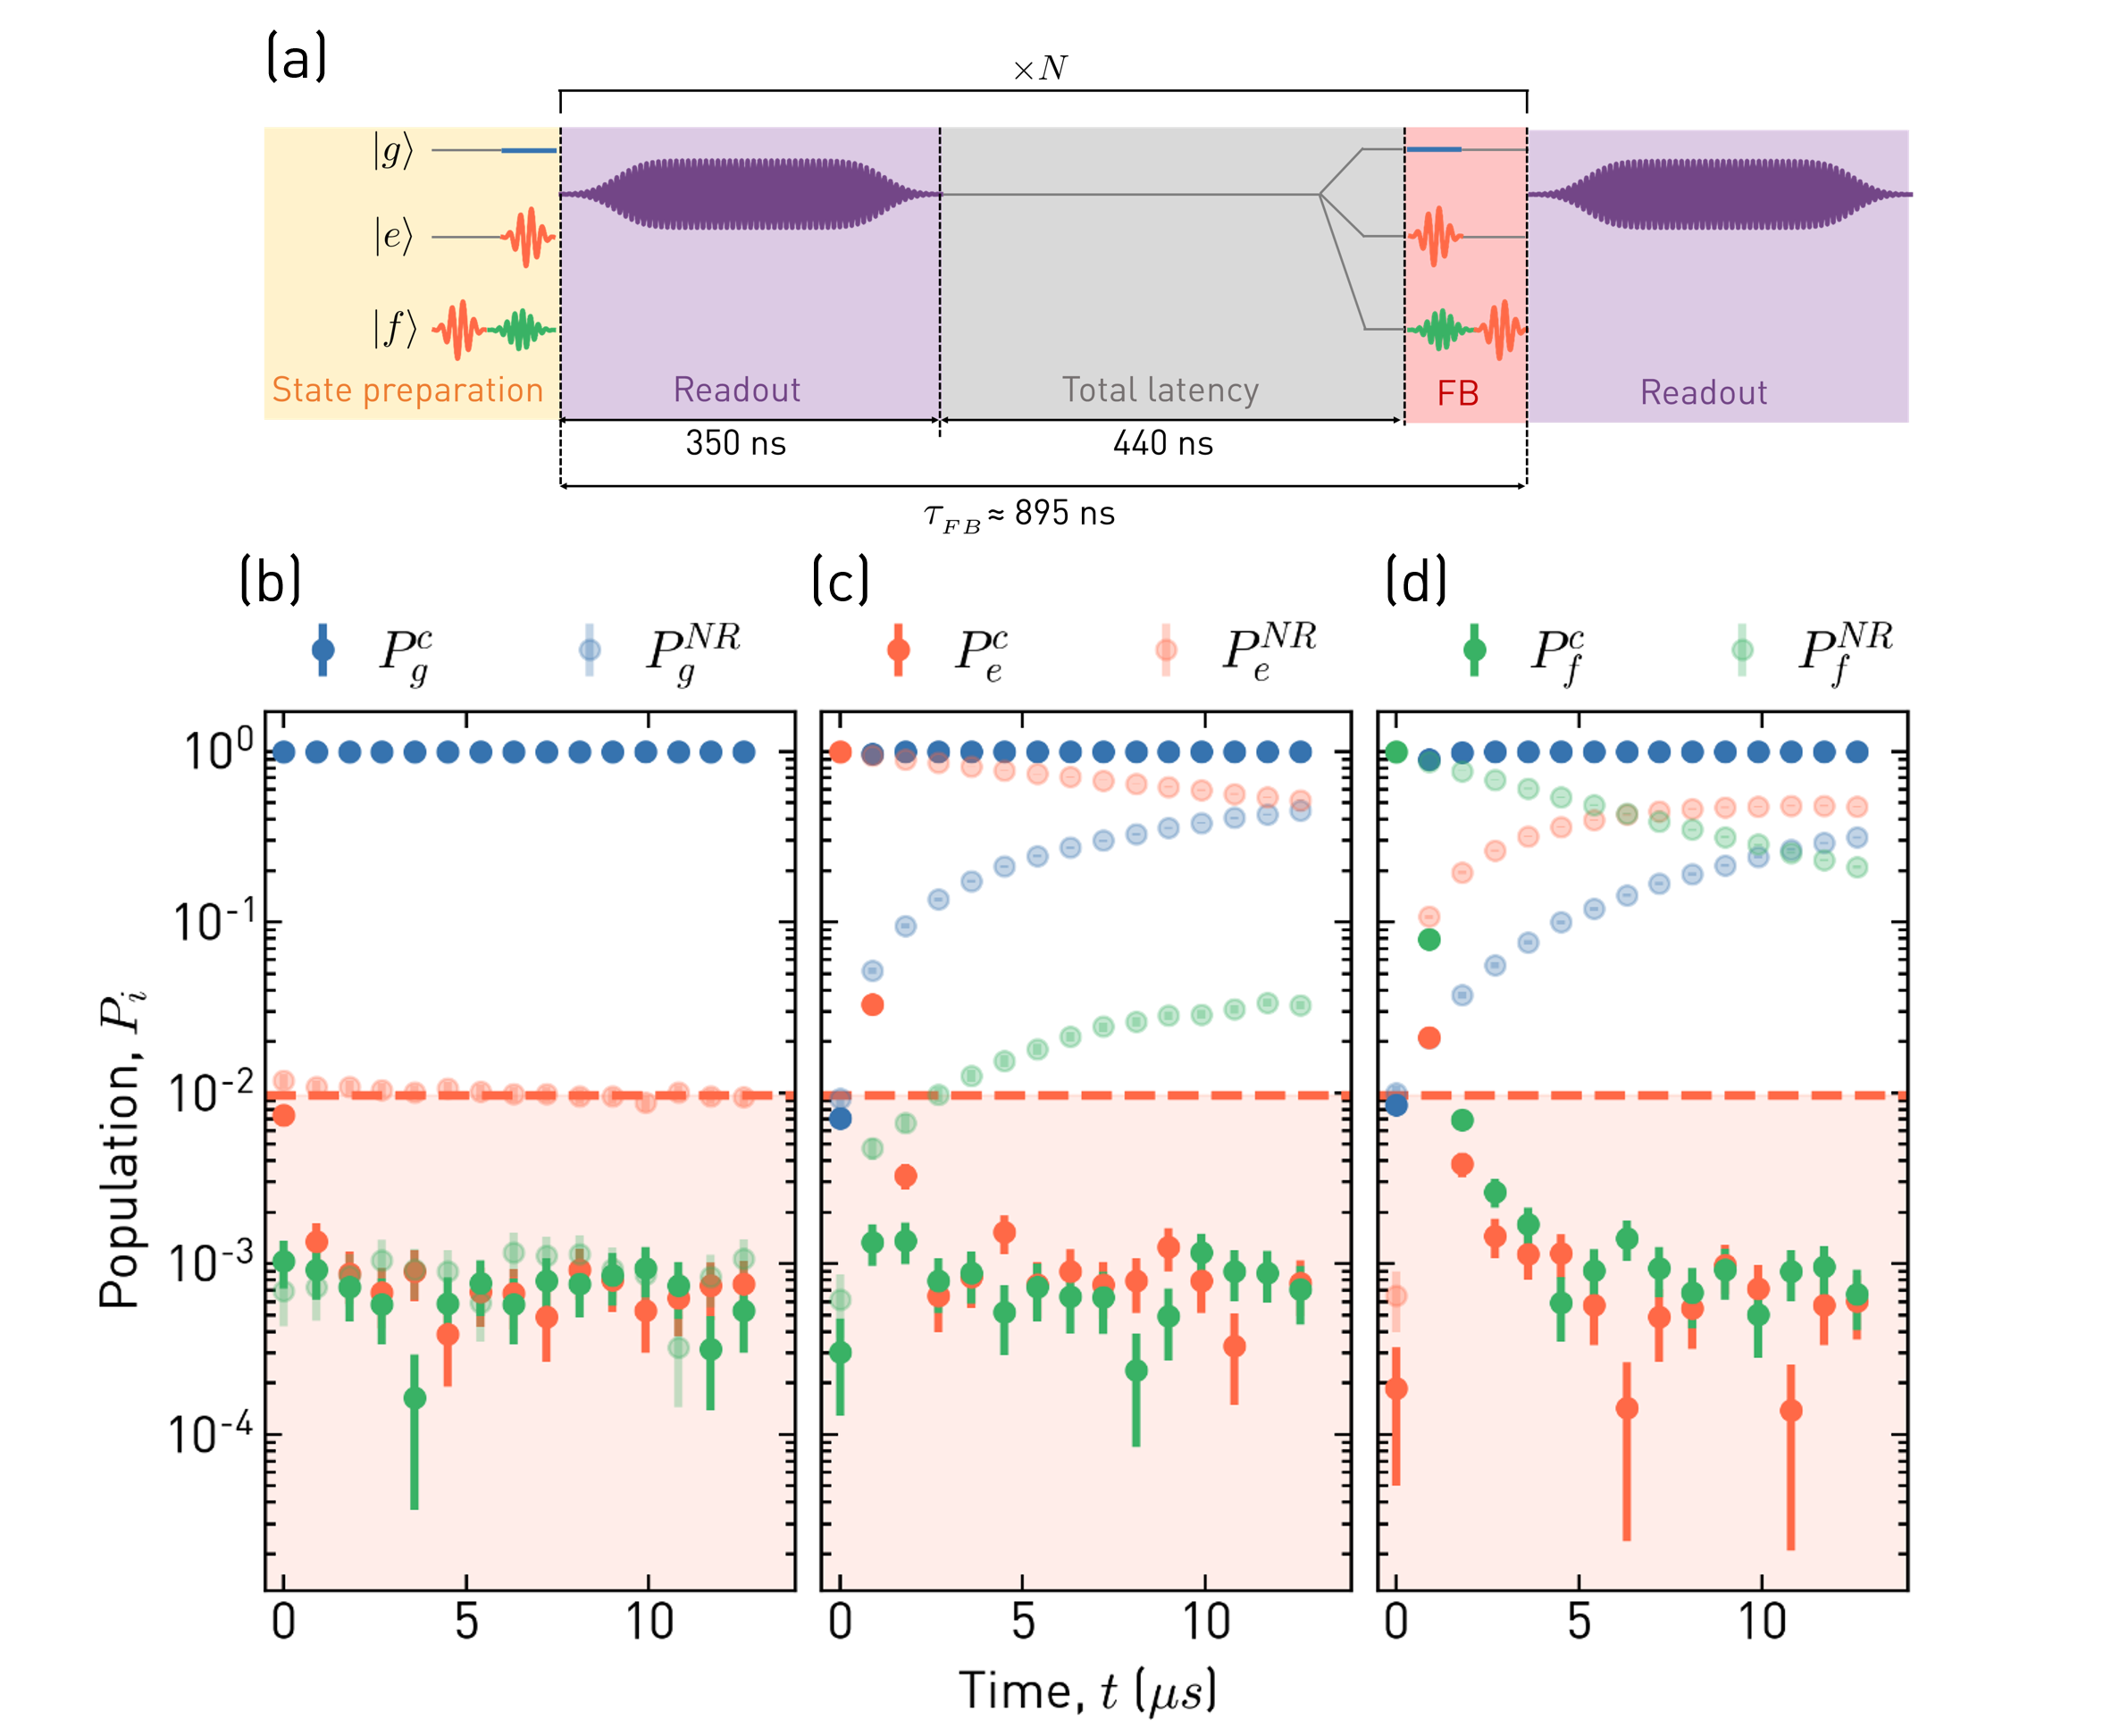
\includegraphics[width=\textwidth]{appendices/qutrit_readout/figs/ch3_readout_active_reset_residual_populations_20200118_175702_with_scheme.png}
    \caption{(a) Pulse scheme used to test the active reset protocol. We prepare a qutrit in one of its eigenstate and subsequently apply $N$ feedback cycles consisting of a readout pulse, a waiting time to assign a state to the acquired data and generate a code word for the \gls{hdawg}, and a feedback sequence to reset the qutrit to the ground state dependent on the code word. Finally, we apply a last readout pulse to evaluate the impact of the last feedback cycle. Single-qubit identity gates $I$ (i.e. wait time) are shown in blue, single-qubit x-rotation in the $ge$-subspace $R_{ge}^{\pi}$ are indicated in red and in red and single-qubit x-rotation in the $ef$-subspace $R_{ef}^{\pi}$ are indicated in green. (b-d) Evolution of the readout-corrected populations $P_{g,e,f}^c$ over time after a state preparation in \g{} (b), \e{} (c) and \f{} (d) of qubit 1. The $n$-th time step corresponds to the $n$-th readout of the reset scheme. The reference measurement recording populations $P_{g,e,f}^{NR}$ without reset pulse is shown with translucent colors in each panel. We indicate the average, steady-state excited population $\langle P_{\textrm{exc}}^{NR}\rangle$ with a dashed red line, and shade the region below this threshold in light red.}
    \label{fig:qutrit_readout_active_reset_populations}
\end{figure}

For a qutrit prepared in \g, about 99\% of the population is measured in \g{} at $t=0$ (i.e. before applying the first feedback pulse), see Fig.~\ref{fig:qutrit_readout_active_reset_populations}(b). The residual excited population originating from thermal excitation amounts to approximately 1\% and is predominantly in the \e-state. After a single feedback cycle, the residual excited population is on the order of $1\permil$, i.e. an order of magnitude smaller, and stays approximately constant thereafter.

Similarly, a qutrit prepared in \e{} starts with approximately 99\% of the population in \e, but requires 2 feedback cycles (1.8\us) to reduce the residual excited population below $\langle P_{\textrm{exc}}^{NR}\rangle$  and 3 cycles (2.7\us) to reach a steady-state of approximately 1.5$\permil$, see Fig.~\ref{fig:qutrit_readout_active_reset_populations}(c). This population transfer occurs about 100 times faster than it would through the natural decay of the qutrit (see translucent data points for comparison). The increase in $P_f^{NR}$ is due to the accumulation of measurement-induced transitions. The ability the readout the \f-state and correct for these excitation results in a constant \f-state population of approximately 1$\permil$ when the feedback is activated.

Finally, we also demonstrate the ability to reset a qutrit prepared in \f{} below $\langle P_{\textrm{exc}}^{NR}\rangle$ with 3 feedback cycles (2.7\us), see Fig.~\ref{fig:qutrit_readout_active_reset_populations}(d).

In Fig.~\ref{fig:qutrit_readout_active_reset_rates}, we present the residual excited state population for a qutrit prepared in \e{} and \f{}, which we fit to a exponential decaying model to extract the reset rate, $\Gamma$, and the residual, steady-state excited population $P_{\textrm{exc}}^{\textrm{ss}}$,
\begin{equation}\label{eq:qutrit_readout_active_reset_rate_model}
    P_{\textrm{exc}} = P_{\textrm{exc}}^{\textrm{ss}} + (1-P_{\textrm{exc}}^{\textrm{ss}}) \cdot \sexp{-2\pi\Gamma t}
\end{equation}

We extract a reset rate of 0.60\unit{MHz} (0.41\unit{MHz}) and a steady-state, residual excited population of 1.5\unit{\permil} (1.7\unit{\permil}) for a qutrit prepared in \e{} (\f). 

\begin{figure}[ht]
    \centering
    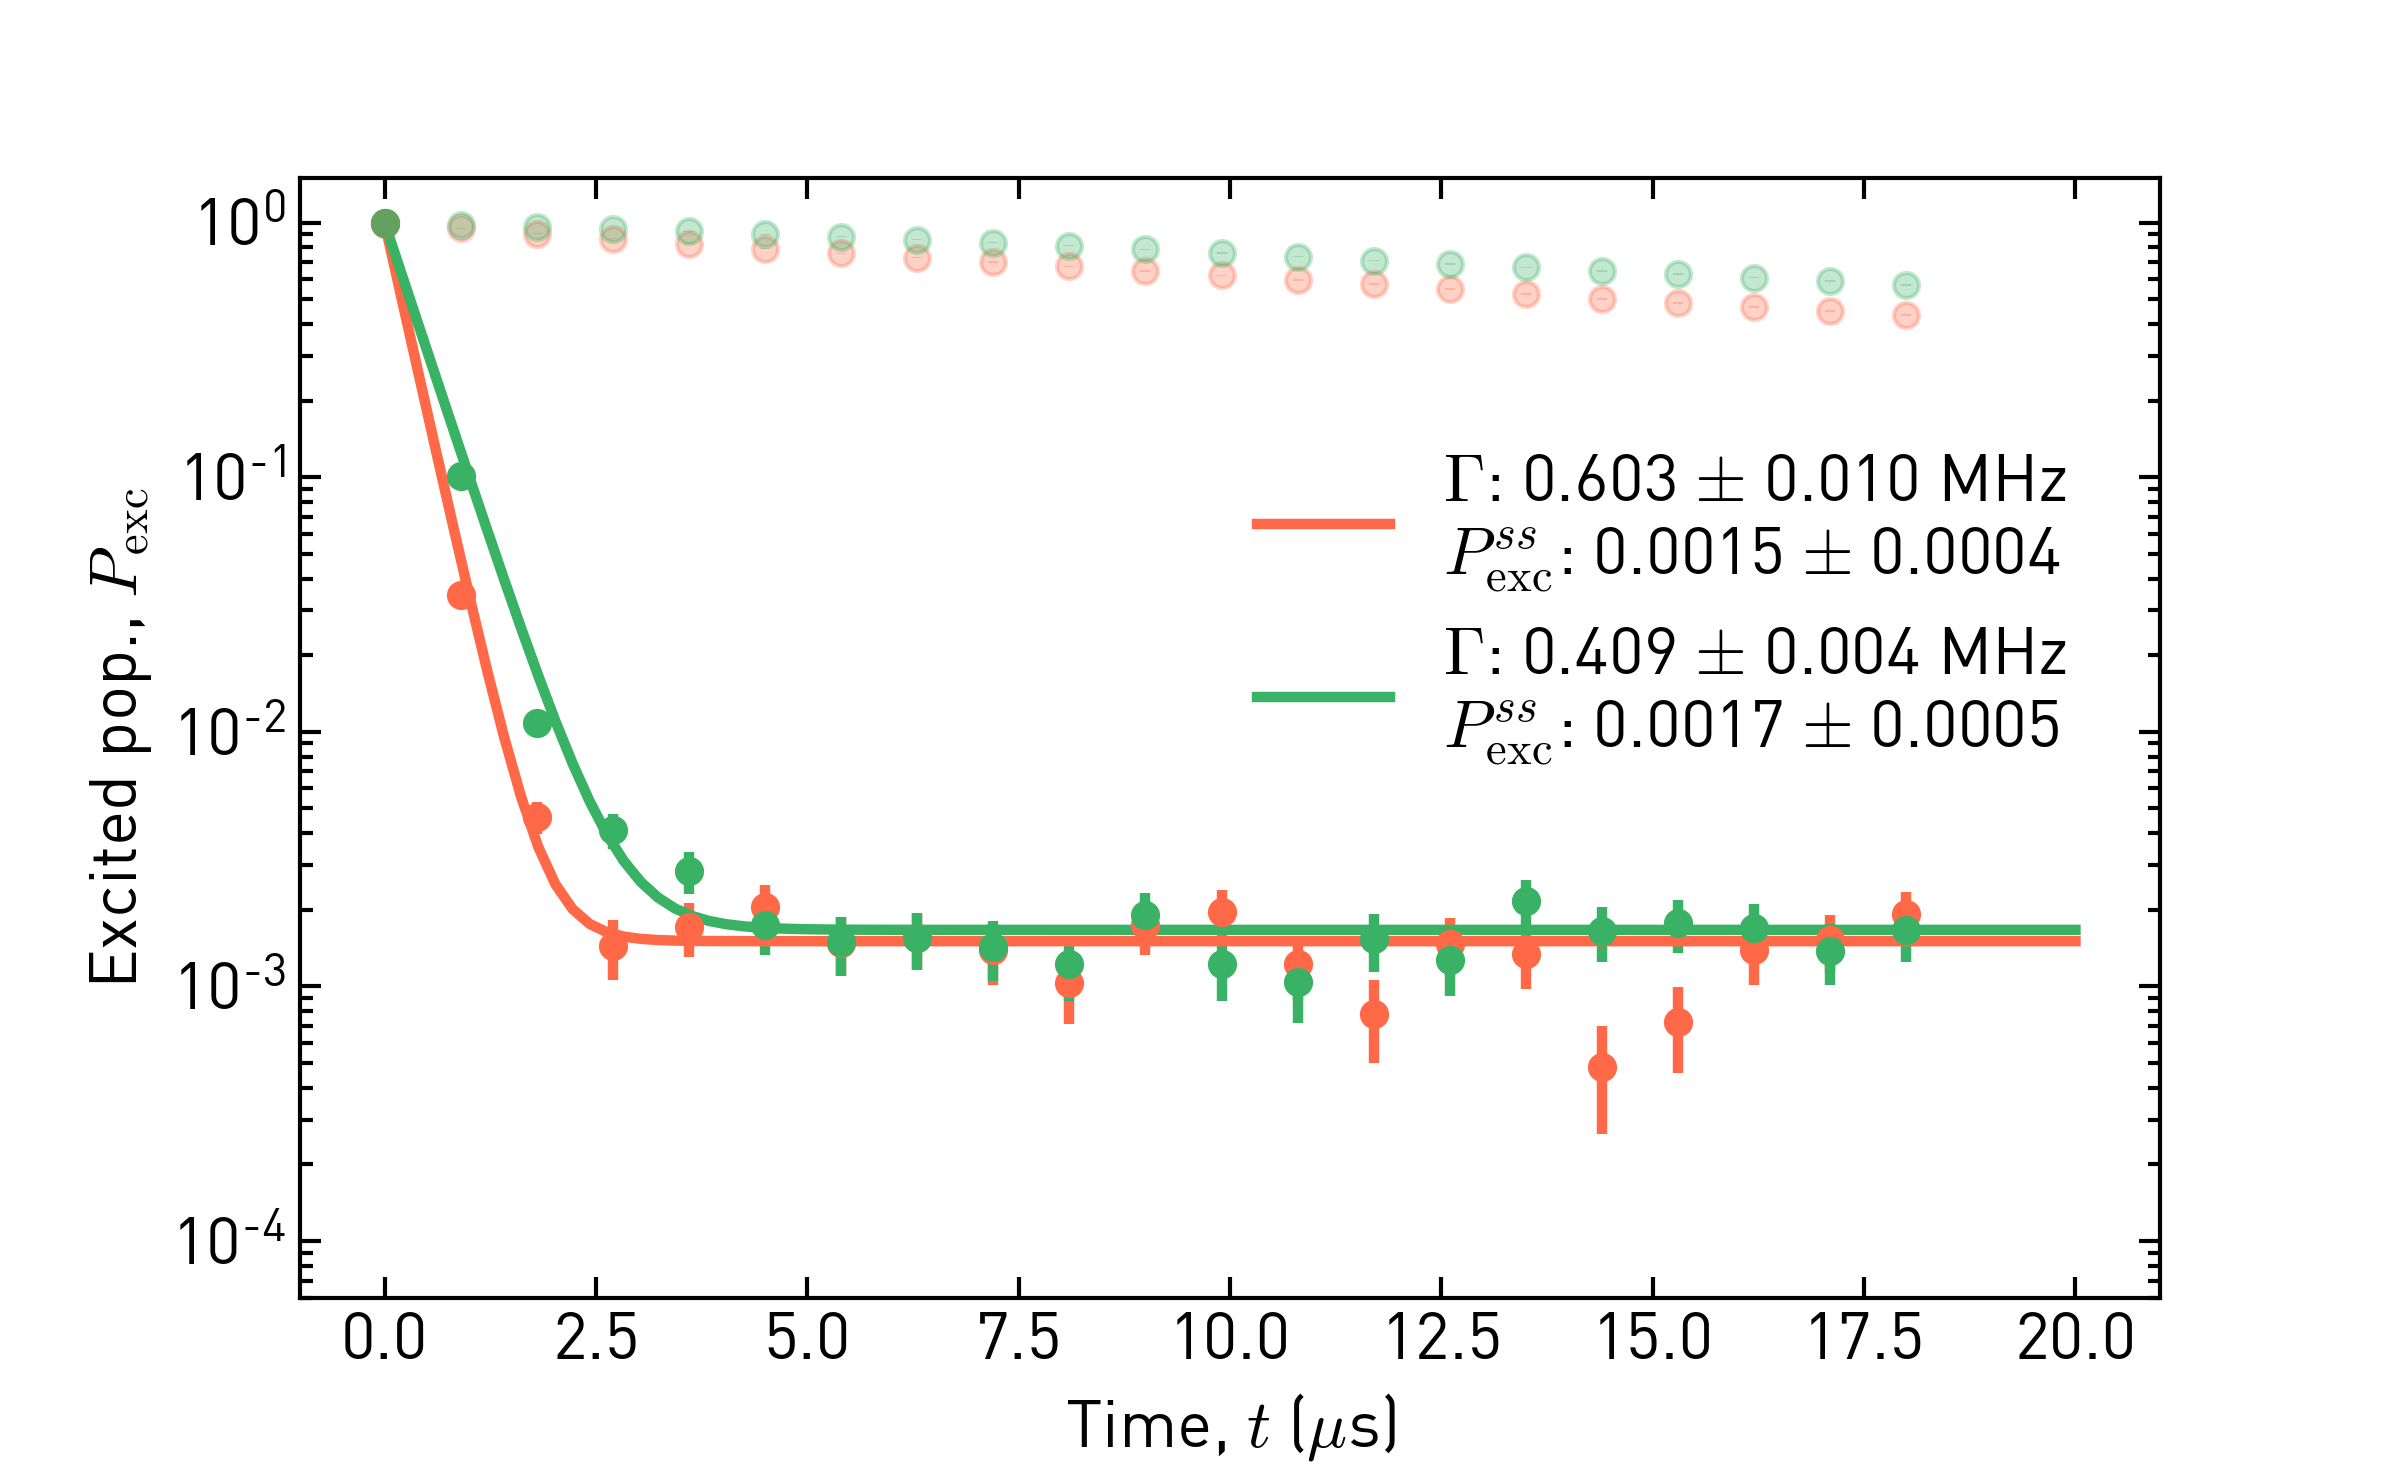
\includegraphics[width=\textwidth]{appendices/qutrit_readout/figs/ch3_readout_active_reset_fit_20200308_173706.png}
    \caption{Excited state population for a qutrit prepared in \e{} (red) and \f{} (green). The solid lines correspond to a fit to Eq.~\eqref{eq:qutrit_readout_active_reset_rate_model} to extract the reset rate and the residual, steady-state excited population. For reference, the excited state population when no reset is applied is shown in translucent colors.}
    \label{fig:qutrit_readout_active_reset_rates}
\end{figure}{}

\subsubsection{Comparison to literature}
In Fig.~\ref{fig:qutrit_readout_reset_rate_comparison}, we extend the comparison of different reset protocols presented in Ref.~\cite{Magnard2018FastQubit} in terms of reset rate and residual, steady-state population to include this work (reset on \e{} only, because not all other reset protocols include reset of \f).

\begin{figure}[ht]
    \centering
    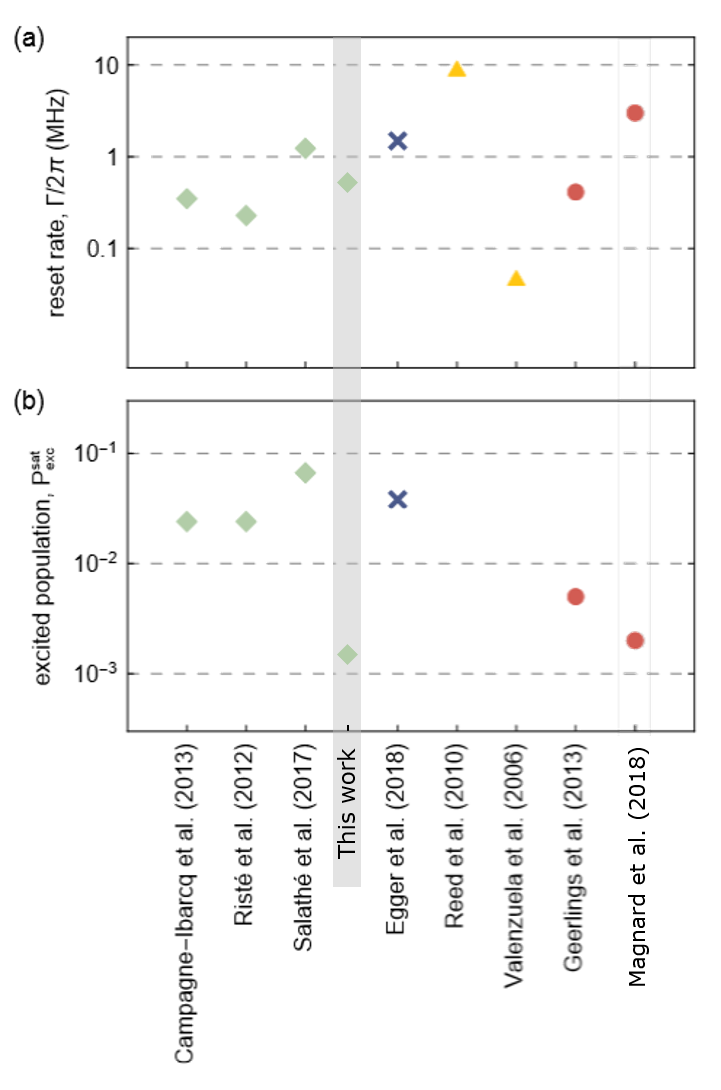
\includegraphics[width=0.5\textwidth]{appendices/qutrit_readout/figs/table_reset_rates.png}
    \caption{Comparison of reset rates $\Gamma$ (a) and residual, steady-state excited populations $P_\textrm{exc}^{ss}$ (b) of various implementations  of  qubit  reset  protocols. The protocol represented with green squares are, similarly to this work, based on qubit measurement and feedback control. We compare additional protocols based on: sequential $\pi$-pulses  to  a  dissipative  state (blue cross), qubit frequency tuning via flux pulses (yellow triangles) and all-microwave drive induced dissipation (red circles). Figure and legend reproduced and adapted from~\cite[Supplementary Material]{Magnard2018FastQubit}.}
    \label{fig:qutrit_readout_reset_rate_comparison}
\end{figure}

\subsubsection{Limitations}
There are two main limitations preventing higher reset rates. The first is the length of the feedback cycle. Indeed, the rates are inversely proportional to the time interval between two readouts: an reduction of 25\% of the feedback cycle yields an increase of 25\% of the reset rate, assuming the proportion of states assigned correctly at each time step stays constant (in fact, the proportion grows, see next paragraphs).

The second limitation on a qutrit prepared in \e{} is the decay between the second half of the readout pulse and the arrival of the feedback pulse. If the qutrit state was correctly labeled as \e{} but has decayed before the feedback pulse is applied, the feedback pulse will set the qutrit state back to \e{}. We expect 2.5-3\% of prepared states to decay during the above-mentioned time interval (615\unit{ns}) for \t{1} of 20-24\us{} which we typically observe for qubit 1. This percentage is consistent with the 3.3\% \e-state population observed after 1 feedback cycle for a qutrit prepared in \e. 

The same phenomenon limits the reset rate on a qutrit prepared in \f, however, the shorter \f-level lifetime results is more decay events within the time interval and hence a slower reset rate. 

Hence, further increase the reset rate requires a reduction of decay events which can be obtained by an increase in qutrit lifetime, or a reduction of the total latency before the feedback pulses are applied, i.e. a faster readout or an optimized \gls{uhf} firmware capable of assigning states faster. 

The main factor limiting the residual, steady-state population is the readout infidelity of the ground state, i.e. the probability of assigning \e{} or \f{} to a qutrit actually in \g. For qubit 1, the readout infidelity is 1.6\unit{\permil} which is in excellent agreement with  the observed $P_\textrm{exc}^{ss}$ of 1.5\unit{\permil} and 1.7\unit{\permil}. 

We can decrease this readout infidelity by shifting the decision thresholds further away from the mean of the ground state distribution to increase the size of the region where a state is labeled as \g{} and decrease errors caused by ground state data point located near the decision boundaries.  The ultimate population limit then becomes the re-thermalization occurring between the readout and the feedback pulse, which amounts to 0.2-0.4\unit{\permil} for qubit 1 on this device. 

Nevertheless, using more conservative thresholds for the ground state comes at a expense of increasing the probability of assigning \g{} to a qutrit actually in \e{} or \f, which in turn decreases the reset rate.

\subsubsection{Conclusion}
In this section, we have implemented a three-level, measurement-based active reset protocol yielding a reset rate of 0.60\unit{MHz} (0.41\unit{MHz}) and a residual, steady-state excited population of 1.5\unit{\permil} (1.7\unit{\permil}) for a qutrit prepared in \e{} (\f).

In addition, this reset protocol can be used at the end of any measurement sequence to reset the qutrit to its ground state, and thereby increase the measurement repetition rate by a factor of 10 compared to waiting for the natural decay of the qutrit.

The main limitation of the reset protocol is the delay between readout and the application of the feedback pulse.

Nevertheless, this reset protocol is competitive with respect to other state-of-the-art protocols and further improvement of readout circuitry, as well as electronics firmware optimization potentially allow yet better performance.




